\documentclass[12pt, a4paper]{report}

\usepackage{Others/preamble}     % your custom style file (already uploaded)
\usepackage{pdfpages}   
\usepackage[round,sort,sectionbib]{natbib}  %  → References heading gets correct size

\usepackage{chapterbib}   % enables a separate .bbl for every \include

% hyperref should come **last**                                    
\usepackage[colorlinks=true,backref=page]{hyperref}
\hypersetup{linkcolor=gray, citecolor=gray, urlcolor=gray}

\title{Microeconomics I Lecture Notes}
\author{Enrico Mattia Salonia}
\date{Latest version: \today \\
This is a first draft of notes that I plan to improve and expand!}  % or a fixed date

% --------------------------------------------------------------------
\begin{document}
% --------------------------------------------------------------------

% --- Roman numerals start; count the title page as i (but don't print it)
\cleardoublepage
\pagenumbering{roman}
\setcounter{page}{1}

% Title page ---------------------------------------------------------
\begin{titlepage}
	\centering
	\makeatletter                   % <— open access to @‑macros
	{\LARGE\bfseries \@title\par}\vspace{2cm}

	%{\Large \textit{A thesis submitted for the degree of Doctor of Philosophy}\par}\vspace{1.5cm}

	%{\Large by\par}\vspace{0.5cm}
	{\Large\bfseries \@author\par}\vspace{0.5cm}  % line 44 — now defined

	{\@date}                        % uses whatever you put in \date{}
	\makeatother                    % <— close @ access
\end{titlepage}

\cleardoublepage

% Roman‑numeral prelims ----------------------------------------------
\pagenumbering{roman}

\cleardoublepage          % or \clearpage   –– finish previous text
\thispagestyle{empty}     % 1. suppress header/footer (hides the number)

% ... any material that belongs on the un-numbered page ...

\addtocounter{page}{-1}

\setcounter{page}{2} % title‑page is p. i
\tableofcontents
\cleardoublepage

% Arabic‑numeral main matter -----------------------------------------
\pagenumbering{arabic}
\chapter*{Preamble}\label{ch:preamble} % no number
\addcontentsline{toc}{chapter}{Preamble} % include in the ToC

These notes accompany the first part of the PhD microeconomics sequence. They cover \textbf{choice under uncertainty} and \textbf{general equilibrium theory}.
The write-up is still a work in progress, and I will continue to update it. If you spot any mistakes or typos, please let me know.

I have aimed for a conversational style rather than the more formal tone of, say, \citet{mas-colellMicroeconomicTheory1995}. I assume no prior knowledge of the topics, though—as usual—some mathematical maturity helps (and I hope you will develop it along the way!). Each lecture summarizes what we cover in class, followed by exercises and suggestions for further reading. Whenever a result is proved, I have tried to give the simplest proof available. This often makes explanations and proofs a bit longer than strictly necessary, but, I hope, also more accessible.

Before diving in, you might enjoy some non-technical background that helps frame the topics we will study: \citet[ch.~1]{krepsNotesTheoryChoice1988}, \citet[pp.~ix–xi]{debreuTheoryValueAxiomatic1959}, \citet[pp.~1–7]{myersonGameTheoryAnalysis1997}, and \citet[chs.~1–2]{gilboaTheoryDecisionUncertainty2009}.

\begin{techremark}
	You will occasionally see smaller text like this. These remarks are not essential for following the main exposition, but they add context or point to related ideas. Feel free to skip them on a first pass.
	\normalsize
\end{techremark}

These notes draw on several sources. The main reference is \citet{mas-colellMicroeconomicTheory1995}, but both here and in the text you will find pointers to alternative or complementary readings. A short reading list follows. If you would like more references or wish to discuss any of the material, just send me an email—I am always happy to talk.



\bigskip

\begin{center}
	\Large Have fun!\normalsize
\end{center}

\bigskip

\noindent
\begin{minipage}[t]{0.48\textwidth}
	\paragraph{Choice under uncertainty.}
	\begin{itemize}
		\item \textbf{\citet{mas-colellMicroeconomicTheory1995}, ch.~6.}
		\item \citet{krepsNotesTheoryChoice1988}, chs.~4-6.
		\item \citet{fishburnUtilityTheoryDecision1970}, ch.~8.
		\item \citet{krepsMicroeconomicFoundations2013}, chs.~5-6.
		\item \citet{gilboaTheoryDecisionUncertainty2009}.
	\end{itemize}
\end{minipage}%
\hfill
\begin{minipage}[t]{0.52\textwidth}
	\paragraph{General equilibrium theory.}
	\begin{itemize}
		\item \textbf{\citet{mas-colellMicroeconomicTheory1995} chs.~15–17.}
		\item \cite{thomsonFairAllocationRules2011}, sec 4.3 (no-envy).
		\item \citet{krepsMicroeconomicFoundations2013}, chs.~14–15.
		\item \citet{debreuTheoryValueAxiomatic1959}.
		\item \citet{hildenbrandIntroductionEquilibriumAnalysis1976}.
	\end{itemize}
\end{minipage}


\bibliographystyle{apacite}
\bibliography{references}

\setcounter{chapter}{0}% <—  important!
\renewcommand{\thefootnote}{\fnsymbol{footnote}}

\chapter[Introduction to Expected Utility]%
 {Introduction to Expected Utility}
\label{ch:L1}

% 3) Reset things so later footnotes go back to 1, 2, 3, …
\setcounter{footnote}{0}
\renewcommand{\thefootnote}{\arabic{footnote}}

\section{How to model uncertainty}\label{sec:L1-intro}

Let's start by thinking about how we represent uncertainty. Say that you made a bet with a friend: if a fair coin toss results in heads, you get \(10\) euros; otherwise you pay \(10\) euros to your friend. There are two outcomes, \(10\) and \(-10\), and since the coin is fair, each occurs with probability \(\nicefrac{1}{2}\). To describe this simple example, we started from a set of outcomes, monetary transfers, and specified the probability of each outcome occurring. I refer to such an object as a \textit{lottery}. Denote the set of outcomes by \(X\). Generic elements of \(X\) will be denoted \(x,y,z\). For now, we assume that \(X\) is finite. Outcomes alone are not enough to describe a lottery: we need probability distributions over outcomes, as in the \(\nicefrac{1}{2}\)–\(\nicefrac{1}{2}\) distribution of the fair coin above. The set of lotteries over \(X\) is denoted by \(\Delta(X)\).\footnote{Wonder why this notation? You will realise soon.} Each element of \(\Delta(X)\) is a function \(p : X \to [0,1]\) such that \(\sum_{x \in X} p(x) = 1\), it maps each outcome \(x\) to a number \(p(x)\) in \([0,1]\), representing the probability that \(x\) occurs.\footnote{Why do we write the sum \(\sum_{x \in X} p(x) = 1\) instead of an integral?}

\begin{example}
	In the example above, the set of outcomes is \(\{10,-10\}\) and the lottery induced by the fair coin toss satisfies \(p(10) = p(-10) = \nicefrac{1}{2}\).
\end{example}

\begin{remark}
	Notice that, in this setup, we are missing something: whether the coin lands on heads or tails is irrelevant; only the probabilities of outcomes matter, not the events that induced them. This is a limitation of this model, which we will address when we introduce a state-space representation of uncertainty.
\end{remark}

We now need to make statements such as \textquote{an individual prefers lottery \(p\) to lottery \(q\).} To do so, we introduce a binary relation \(\succsim\) over \(\Delta(X)\), so that \(p \succsim q\) means that the individual weakly prefers lottery \(p\) to lottery \(q\). Compared to choice under certainty, we are now comparing lotteries—i.e., probability distributions over outcomes—rather than outcomes themselves. The set we are ranking, the set of lotteries, has \emph{structure}, whereas the set of outcomes does not. For example, we can consider a lottery \(r\) that yields \(p\) with probability \(\alpha\) and \(q\) with probability \(1-\alpha\), where \(\alpha \in [0,1]\). This is called a \textit{compound lottery}, and it is an element of \(\Delta(X)\) as well, we can write \(r = \alpha p + (1-\alpha) q\). For instance, if \(p(10)=1\) and \(q(-10)=1\), then \(r(10) = \alpha\) and \(r(-10) = 1-\alpha\). This \emph{mixing} operation is generally not possible with an unstructured set of outcomes. As an illustration, suppose the set of outcomes comprises fruits. We can have an apple or a banana, but there is no fruit that is a mixture of an apple and a banana. Imposing structure on the set of elements to be ranked is a key move of microeconomic theory. In fact, we will later assume that the set of outcomes is \(\mathbb{R}\), the set of real numbers representing monetary outcomes, allowing us to say more than what we can say with a generic set of outcomes.

\begin{techremark}
	Technically, \(\succsim\) is a subset of \(\Delta(X) \times \Delta(X)\), i.e., a set of ordered pairs of lotteries. For example, if \(p,q,r \in \Delta(X)\), the individual prefers \(p\) to \(q\), and is indifferent between \(q\) and \(r\), then \(\succsim\) contains at least the pairs \((p,q),(q,r),(p,r),(p,p),(q,q),(r,r)\).
\end{techremark}

In what follows, we consider what assumptions preferences over lotteries might satisfy, and what these assumptions imply.

\section{Things to read}

Check \citet[p. 31-33]{krepsNotesTheoryChoice1988} for an introduction of the lottery model in this chapter.

\section{Exercises}

Some exercises here.

\begin{exercise}
	Nice exercise.
\end{exercise}

\bibliographystyle{apacite}  % or another  style
\bibliography{references} % .bib file goes in ./bib/
\renewcommand{\thefootnote}{\fnsymbol{footnote}}

\chapter[Expected utility theory]%
 {Expected utility theory}
\label{ch:L2}

% 3) Reset things so later footnotes go back to 1, 2, 3, …
\setcounter{footnote}{0}
\renewcommand{\thefootnote}{\arabic{footnote}}

\section{Ciao}\label{sec:L2-intro}

Let's talk about axioms.

\begin{axiom}\label{ax:wo}
	\labelname{axn:wo}{Weak order} (\textbf{Weak order}) Preferences \(\succsim_i\) are complete, transitive and continuous.
\end{axiom}

\usename{axn:wo}





\cite{aczelLecturesFunctionalEquations1966} come va.

\section{Things to read}

ciao

\section{Exercises}

\begin{exercise}
    Ciao.
\end{exercise}

\bibliographystyle{apacite}  % or another  style
\bibliography{references} % .bib file goes in ./bib/
\renewcommand{\thefootnote}{\fnsymbol{footnote}}

\chapter[Money lotteries]%
 {Money lotteries}%
\label{ch:L3}

% 3) Reset things so later footnotes go back to 1, 2, 3, …
%\setcounter{footnote}{0}
\renewcommand{\thefootnote}{\arabic{footnote}}

\section{Structuring the set  of outcomes}\label{sec:L3-intro}

In the previous section, we studied preferences with the expected utility form over lotteries on a \textit{finite} outcome set \( X \). We now study a setting where the outcome set is the set of real numbers \( \mathbb{R} \), representing monetary outcomes. This setting is particularly important in economics and finance, as it allows us to model decisions involving money, such as investments, insurance, and consumption choices.

\begin{techremark}
	You may wonder wether a form of Theorem \ref{thm:eu} can be extended to such a setting. The answer is yes, if you are interested check \citet[pp. 59-78]{krepsNotesTheoryChoice1988} or \citet[ch. 10]{fishburnUtilityTheoryDecision1970}.
\end{techremark}

Since the outcome set is now infinite, we need to be careful about how we define lotteries. We introduce cumulative distribution functions (CDFs) to represent lotteries over monetary outcomes. A CDF \( F: \mathbb{R} \to [0, 1] \) maps each monetary outcome \( x \) to the probability that the outcome is less than or equal to \( x \). It satisfies the following properties:
\begin{itemize}
	\item \( F \) is non-decreasing: if \( x \leq y \), then \( F(x) \leq F(y) \).
	\item \( \lim_{x \to -\infty} F(x) = 0 \) and \( \lim_{x \to +\infty} F(x) = 1 \).
	\item \( F \) is right-continuous, i.e. for every \( x \in \mathbb{R} \), \( \lim_{y \downarrow x} F(y) = F(x) \).\footnote{The symbol \(y \downarrow x\) means that \(y\) approaches \(x\) from above.}
\end{itemize}


\begin{example}
	Consider a lottery that pays 1 dollar with probability \( \tfrac14 \), 4 dollars with probability \( \tfrac12 \), and 6 dollars with probability \( \tfrac14 \). The corresponding CDF \( F \) is given by:

	\[
		F(x) =
		\begin{cases}
			0        & \text{if } x < 1,        \\
			\tfrac14 & \text{if } 1 \leq x < 4, \\
			\tfrac34 & \text{if } 4 \leq x < 6, \\
			1        & \text{if } x \geq 6,
		\end{cases}
	\]

	it is represented in Figure \ref{fig:cdf_example}.

	\begin{figure}[H]
		\centering
		\begin{tikzpicture}[x=1cm,y=5cm,>=stealth]
			% Axes
			\draw[->] (0,0) -- (9,0) node[below right] {$x$};
			\draw[->] (0,0) -- (0,1.15) node[above left] {$F(\,\cdot\,)$};

			% y-ticks and labels
			\foreach \y/\lab in {0.25/{$\tfrac14$}, 0.75/{$\tfrac34$}, 1/{$1$}}{
			\draw (-0.07,\y) -- (0.07,\y);
			\node[left] at (-0.07,\y) {\lab};
			}

			% x-ticks and labels
			\foreach \x/\lab in {1/{1 dollar}, 4/{4 dollars}, 6/{6 dollars}}{
			\draw (\x,0.03) -- (\x,-0.03);
			\node[below] at (\x,-0.03) {\lab};
			}

			% Dashed guide at F=1 (optional)
			\draw[dashed,gray] (0.2,1) -- (6,1);

			% Step function segments (right-continuous) — BLUE
			% Including the flat part from 0 to 1 dollar
			\draw[blue,line width=1.0pt] (0,0) -- (1,0);
			\draw[blue,line width=1.0pt] (1,0.25) -- (4,0.25);
			\draw[blue,line width=1.0pt] (4,0.75) -- (6,0.75);
			\draw[blue,line width=1.0pt] (6,1) -- (8.8,1) node[right,text=blue] {$F(\cdot)$};

			% Open circles at left limits (showing jumps)
			\draw[fill=white, line width=0.8pt] (1,0) circle (2pt);
			\draw[fill=white, line width=0.8pt] (4,0.25) circle (2pt);
			\draw[fill=white, line width=0.8pt] (6,0.75) circle (2pt);

			% Closed (filled) circles at right-continuous values
			\fill (1,0.25) circle (2pt);
			\fill (4,0.75) circle (2pt);
			\fill (6,1.0)   circle (2pt);
		\end{tikzpicture}

		\caption{Cumulative distribution function (CDF) representing a lottery over monetary outcomes.}
		\label{fig:cdf_example}
	\end{figure}
\end{example}

Notice that mixtures of CDFs are also CDFs, so we can employ the same mixture operation defined in Section \ref{sec:L1-intro}. In particular, given two CDFs \( F \) and \( G \), and \( \alpha \in [0, 1] \), the mixture \( H = \alpha F + (1 - \alpha) G \) is also a CDF, where \( H(x) = \alpha F(x) + (1 - \alpha) G(x) \) for all \( x \in \mathbb{R} \).

We now define preferences \( \succsim \) over the set of CDFs over non-negative amounts of money that have the expected utility form. The idea is the same, we weight the utility of each monetary outcome by its probability, and sum these weighted utilities to get the expected utility of the lottery. Formally, a preference relation \( \succsim \) over the set of CDFs has the expected utility form if there exists a utility function \( u: \mathbb{R} \to \mathbb{R} \) such that for any two CDFs \( F \) and \( G \):

\[
	F \succsim G \quad \text{if and only if} \quad \int u(x)dF(x) \geq \int u(x)dG(x).
\]

Before we had a utility function over outcomes \( u : X \rightarrow \), but now the set of outcomes is \( \mathbb{R} \), that is why the domain is different. Such distinction allows us to introduce properties of the function \( u \) that are specific to monetary outcomes. From now on, we assume the following two.

\begin{definition}\label{def:increasing}
	The utility function \( u \) is \textbf{increasing} if for any \( x, y \) such that \( x > y \), we have \( u(x) > u(y) \).
\end{definition}

Definition \ref{def:increasing} captures the idea that more money is always preferred to less money. When the outcome set was \( X \), we could not state this property, as \( x > y \) meant nothing.\footnote{As an example, if \( x \) is an apple and \( y \) is a banana, what does \( x > y \) means?}

\begin{definition}\label{def:continuity}
	The utility function \( u \) is \textbf{continuous} if for any \( x \) and any \( \varepsilon > 0 \), there exists a \( \delta > 0 \) such that for all \( y \) with \( |x - y| < \delta \), we have \( |u(x) - u(y)| < \varepsilon \).
\end{definition}

Definition \ref{def:continuity} ensures that small changes in monetary outcomes lead to small changes in utility. This property could not be stated with a generic outcome set, as \( x - y \) had no meaning.

\begin{techremark}
	Definition \ref{def:continuity} is continuity in \textit{money}. What about continuity in probability?
\end{techremark}

\section{Risk aversion}

We now have the tools to define and discuss the concept of risk aversion. Defining this concept allows us to answer the question: how much does an individual dislike risk? As we will see, the answer to this question has important implications for economic behavior, such as investment decisions and insurance choices.

The definition of risk aversion is quite intuitive. Consider an individual offered the following opportunity: they can either receive \( 5 \) euros, or a lottery that pays \( 0 \) euros with probability \( 0.5 \) and \( 10 \) euros with probability \( 0.5 \). Both options have the same expected monetary value of \( 5 \) euros. Intuitively, if the individual prefers to receive the certain amount of \( 5 \) euros over the lottery, he dislikes risk, prefers getting the mean outcome for sure rather than facing uncertainty. Instead, if the individual prefers the lottery, he likes risk, as he is willing to face uncertainty for the chance of getting a lower payoff.

For each lottery, we define an individual as risk averse if he prefers the certain amount equal to the expected value of the lottery over the lottery itself, as in the example above. For each CDF \( F \), the expected value of the lottery is given by:

\begin{equation}\label{eq:ev}
	\int x dF(x).
\end{equation}

An individual evaluates money using the utility function \( u \). Therefore, the certain amount equal to the expected value of the lottery provides utility

\begin{equation}\label{eq:eu_certain}
	u\left( \int x dF(x) \right).
\end{equation}

On the other hand, the lottery itself provides expected utility

\begin{equation}\label{eq:eu_lottery}
	\int u(x) dF(x).
\end{equation}

We say an individual is risk averse if his utility function \( u \) is such that, for each CDF \( F \), Equation \eqref{eq:eu_certain} is greater than or equal to Equation \eqref{eq:eu_lottery}.

\begin{definition}\label{def:raversion}
	An individual with expected utility preferences and utility function \( u \) is \textbf{risk averse} if for each CDF \( F \)

	\begin{equation}\label{eq:risk_aversion}
		u\left( \int x dF(x) \right) \geq \int u(x) dF(x).
	\end{equation}
\end{definition}

\begin{techremark}
	You should notice that, if \( u \) is not increasing (Definition \ref{def:increasing}), such definition of risk aversion does not make sense.
\end{techremark}

Equation \eqref{eq:risk_aversion} is \href{https://en.wikipedia.org/wiki/Jensen%27s_inequality}{Jensen's inequality}, and it defines concavity of the utility function \( u \). Therefore, the intuitive notion of risk aversion we discussed is technically equivalent to concavity of \( u \), as illustrated in Figure \ref{fig:risk_aversion}. Recall that concavity of \( u \), if it is twice differentiable, means that its second derivative is non-positive, i.e. \( u''(x) \leq 0 \) for all \( x \).

\begin{figure}[H]
	\centering
	\tikzset{every picture/.style={line width=0.75pt}} %set default line width to 0.75pt        
	\begin{tikzpicture}[x=0.65pt,y=0.65pt,yscale=-1,xscale=1]
		%uncomment if require: \path (0,433); %set diagram left start at 0, and has height of 433

		%Shape: Axis 2D [id:dp5660095663202026] 
		\draw  (132,370.34) -- (506,370.34)(169.4,62) -- (169.4,404.6) (499,365.34) -- (506,370.34) -- (499,375.34) (164.4,69) -- (169.4,62) -- (174.4,69)  ;
		%Curve Lines [id:da9973639319692577] 
		\draw    (169.4,370.34) .. controls (172,276.6) and (342,108.6) .. (483,108.6) ;
		%Straight Lines [id:da04174830964198639] 
		\draw  [dash pattern={on 4.5pt off 4.5pt}]  (430,370) -- (432,115.8) ;
		%Straight Lines [id:da5426175275814586] 
		\draw  [dash pattern={on 0.84pt off 2.51pt}]  (169.4,370.34) -- (432,115.8) ;
		%Straight Lines [id:da33225594312232143] 
		\draw  [dash pattern={on 4.5pt off 4.5pt}]  (301,370.8) -- (300,181.8) ;
		%Straight Lines [id:da6848091186315952] 
		\draw  [dash pattern={on 4.5pt off 4.5pt}]  (169,243.4) -- (300.7,243.07) ;

		% Text Node
		\draw (422,372.4) node [anchor=north west][inner sep=0.75pt]    {$10$};
		% Text Node
		\draw (510,369.4) node [anchor=north west][inner sep=0.75pt]    {$x$};
		% Text Node
		\draw (403,89.4) node [anchor=north west][inner sep=0.75pt]    {$u( 10)$};
		% Text Node
		\draw (155,372.4) node [anchor=north west][inner sep=0.75pt]    {$0$};
		% Text Node
		\draw (296,372.4) node [anchor=north west][inner sep=0.75pt]    {$5$};
		% Text Node
		\draw (279,148.4) node [anchor=north west][inner sep=0.75pt]    {$u( 5)$};
		% Text Node
		\draw (18,223.4) node [anchor=north west][inner sep=0.75pt]    {$\tfrac{1}{2} u( 0) \ +\ \tfrac{1}{2} u( 10)$};

	\end{tikzpicture}
	\caption{Example of a \( u \) exhibiting risk aversion.}
	\label{fig:risk_aversion}

\end{figure}

Equivalently, an individual is risk loving if the inequality in Definition \ref{def:raversion} is reversed, and risk neutral if the individual is indifferent between the certain amount and the lottery, i.e. if the inequality holds with equality.

There are other ways of defining risk aversion starting from different thought experiments that are equivalent to Definition \ref{def:raversion}. This is good news, it means the definition makes sense! If you are interested in other ways of defining risk aversion, check \citet[p. 186-187]{mas-colellMicroeconomicTheory1995}. We consider another one here. Define the \textbf{certainty equivalent} of a lottery as the certain amount of money that provides the same utility as the lottery itself. That is, the individual must be indifferent between receiving the certainty equivalent for sure and facing the lottery.

\begin{definition}\label{def:ce}
	The \textbf{certainty equivalent} of a lottery with CDF \( F \) for an individual with utility function \( u \) is defined as the solution to the equation

	\begin{equation}\label{eq:ce}
		u(c(F,u)) = \int u(x) dF(x).
	\end{equation}
\end{definition}

Intuitively, if an individual is risk averse, his certainty equivalent must be less than the expected value of the lottery, as he prefers receiving the expected value for sure rather than facing the lottery. To capture this intuition we can define the \textbf{risk premium} of a lottery as the difference between the expected value of the lottery and its certainty equivalent.

\begin{definition}
	The \textbf{risk premium} of a lottery with CDF \( F \) for an individual with utility function \( u \) is

	\begin{equation}\label{eq:rp}
		\pi(F,u) = \int x dF(x) - c(F,u).
	\end{equation}
\end{definition}

You should show in Exercise \ref{ex:cerp} that an individual is risk averse if and only if the risk premium is non-negative for each lottery.

We now have a notion of risk aversion, but not a quantitative measure, which we will develop next. Again, we start from intuition, how could we measure risk aversion? The risk premium might be a starting point, the higher the risk premium, the more risk averse the individual, as he requires a lower certainty equivalent to face the lottery. Consider two individuals with utility function \( u \) and \( v \). If for each lottery \( F \), the risk premium of the first individual is higher than that of the second, i.e. \( \pi(F,u) \geq \pi(F,v) \), we can say that the first individual is more risk averse than the second. However, such condition boils down to comparing certainty equivalents:

\[\pi(F,u) \geq \pi(F,v) \iff c(F,u) \leq c(F,v) \text{ for each lottery } F,\]

you should show this. We therefore have the following definition.

\begin{definition}\label{def:compare}
	An individual with utility function \( u \) is \textbf{more risk averse} than an individual with utility function \( v \) if for each lottery \( F \)

	\[
		c(F,u) \leq c(F,v).
	\]
\end{definition}

We now want to develop a measure of risk aversion that is related to the rate at which the certainty equivalent changes as we change the lottery. Consider a lottery over monetary outcomes that pays \(x + \varepsilon\) with probability \(1/2\) and \(x - \varepsilon\) with probability \(1/2\), call it \(F_\varepsilon\). By Definition~\ref{def:ce}

\begin{equation}\label{eq:ce_eps}
	u\!\big(c(F_\varepsilon,u)\big)
	= \tfrac{1}{2}u(x+\varepsilon) + \tfrac{1}{2}u(x-\varepsilon).
\end{equation}

Since both sides of Equation \eqref{eq:ce_eps} are twice differentiable in \(\varepsilon\) and \(u'(c(F_\varepsilon,u))>0\) since \( u \) is increasing, the implicit function theorem implies that \(c(F_\varepsilon,u)\) is twice differentiable in a neighborhood of \(0\). Differentiating \eqref{eq:ce_eps} with respect to \(\varepsilon\) gives

\[
	u'\!\big(c(F_\varepsilon,u)\big)\,c'(\varepsilon)
	= \tfrac{1}{2}u'(x+\varepsilon) - \tfrac{1}{2}u'(x-\varepsilon).
\]

Evaluating at \(\varepsilon = 0\),

\[
	u'(x)\,c'(0) = 0 \quad \Longrightarrow \quad c'(0) = 0,
	\qquad c(0) = x.
\]

Differentiating again with respect to \(\varepsilon\),

\[
	u''\!\big(c(F_\varepsilon,u)\big)\!\big(c'(\varepsilon)\big)^2
	+ u'\!\big(c(F_\varepsilon,u)\big)c''(\varepsilon)
	= \tfrac{1}{2}u''(x+\varepsilon) + \tfrac{1}{2}u''(x-\varepsilon).
\]

Evaluating at \(\varepsilon = 0\) and using \(c'(0)=0\) and \(c(0)=x\), we obtain

\[
	u'(x)c''(0) = u''(x)
	\quad \Longrightarrow \quad
	c''(0) = \frac{u''(x)}{u'(x)}.
\]

The ratio between the second and first derivative of the utility function is the \textbf{Arrow-Pratt coefficient of absolute risk aversion}. It is not by chance that it appears here. As we noticed already, risk aversion is related to the concavity of the utility function, which is captured by its second derivative. In principle we could use the second derivative alone as a measure of risk aversion, but this would not be satisfactory, as multiplying the utility function by a positive constant would change the second derivative but not risk aversion. Dividing the second derivative by the first derivative solves this problem, as multiplying the utility function by a positive constant multiplies both derivatives by the same constant, leaving their ratio unchanged. The simplest modification of the measure to address such issue is to divide the second derivative by the first derivative, leading to the Arrow-Pratt coefficient.

\begin{definition}\label{def:ap}
	The \textbf{Arrow-Pratt coefficient of absolute risk aversion} for an individual with utility function \( u \) at outcome \( x \) is

	\[
		r(x,u) = -\frac{u''(x)}{u'(x)}.
	\]
\end{definition}

Hence, we just showed that the limit of the second derivative of the certainty equivalent as \(\varepsilon \to 0\) is exactly \(-r(x,u)\). In the exercises, you are asked to show the following equivalence between certainty equivalents and the Arrow-Pratt coefficient.

\begin{proposition}\label{prop:equiv}
	An individual with utility function \( u \) is \textbf{more risk averse} than an individual with utility function \( v \) if and only if for each \( x \)

	\[
		r(x,u) \geq r(x,v),
	\]

	where \( r(x,u) \) and \( r(x,v) \) are the Arrow-Pratt coefficients of absolute risk aversion for individuals with utility functions \( u \) and \( v \).
\end{proposition}

\paragraph{Things to read.} This section mostly draws from \citet[ch. 6.C]{mas-colellMicroeconomicTheory1995}. Alternatives treatments can be found in \citet[ch. 6]{krepsNotesTheoryChoice1988} and \citet[ch. 6]{krepsMicroeconomicFoundations2013}.

\section{Exercises}

\begin{exercise}
	Check that the CDF in Figure \ref{fig:cdf_example} satisfies the three properties of a CDF.
\end{exercise}

\begin{exercise}\label{ex:cerp}
	Show that, if an individual with expected utility preferences and utility function \( u \) is risk averse, his risk premium is non-negative for each lottery.
\end{exercise}

\begin{exercise}
	Prove Proposition \ref{prop:equiv}. (If you are stuck, check \cite{krepsMicroeconomicFoundations2013} or exercises 6.C.6 and 6.C.7 in \citet{mas-colellMicroeconomicTheory1995}.)
\end{exercise}

\bibliographystyle{apacite}  % or another  style
\bibliography{references} % .bib file goes in ./bib/
\renewcommand{\thefootnote}{\fnsymbol{footnote}}

\chapter[Applications and stochastic dominance]%
 {Applications and stochastic dominance}%
\label{ch:L4}

% 3) Reset things so later footnotes go back to 1, 2, 3, …
%\setcounter{footnote}{0}
\renewcommand{\thefootnote}{\arabic{footnote}}

\section{Applications}\label{sec:L4-intro}

come va.

\section{Stochastic dominance}

\paragraph{Things to read.} leggi \cite{mas-colellMicroeconomicTheory1995}.

\section{Exercises}

\begin{exercise}
	ciao ciao
\end{exercise}

\bibliographystyle{apacite}  % or another  style
\bibliography{references} % .bib file goes in ./bib/
\renewcommand{\thefootnote}{\fnsymbol{footnote}}

\chapter[States and subjective expected utility]%
 {States and subjective expected utility}%
\label{ch:L5}

% 3) Reset things so later footnotes go back to 1, 2, 3, …
%\setcounter{footnote}{0}
\renewcommand{\thefootnote}{\arabic{footnote}}

\section{State space representation}\label{sec:L5-intro}

Until now we studied a framework of uncertainty in which the underlying state generating the probability of outcomes was not modelled explicitly, as discussed in Remark \ref{rem:lottery-representation}. There are two advantages of modelling uncerlying states of the world explicitly. The first is that the individual might care about the state \textit{per se}. Consider the following example.

\begin{example}\label{ex:states}
	The birthday of your child is coming up. The problem is that you do not know whether it will rain or be sunny that day. You are a sophisticated parent who offers him monetary bets on the climate whose payoffs he can spend on his birthday party. If it is sunny, he will have a great time playing outside with his friends, while if it rains he will be obliged to organise something indoors. Therefore, he may enjoy each euro spent on his birthday more when it is sunny than when it is raining: his preferences over money depend on the weather.\footnote{The example is inspired by \cite{tsakasBeliefIdentificationProxy2025}}
\end{example}

The first advantage of modelling states explicitly is that it allows us to capture preferences that depend on the state of the world, as in Example \ref{ex:states}. There is a second advantage of modelling states explicitly, but it is easier to explain after we introduce the framework. As in Lecture \ref{ch:L1}, there is a finite set of outcomes \( X \), in Example \ref{ex:states} these are the amounts of money the child could get. Moreover, there is a finite set of mutually exclusive states of the world \( S \). In Example \ref{ex:states}, these are the weather conditions, rain or sun. The individual chooses an \textbf{act}, which is a function from states to outcomes \( f: S \to X \). Act \( f \) in state \( s \) leads to the outcome \( f_s \). In Example \ref{ex:states}, an act is a state-contingent bet. If it rains, the child gets \( f_{\text{rain}} \) euros, while if it is sunny he gets \( f_{\text{sun}} \) euros. Acts are referred to as \textbf{Savage acts}, after \cite{savageFoundationsStatistics1972},\footnote{The first edition was published in 1954.} who introduced the framework and derived subjective expected utility in Definition \ref{def:seu} below.

We can now discuss the second advantage of modelling states explicitly. In Lecture \ref{ch:L1}, the individual chooses among lotteries, probability distributions over outcomes. From individual preferences over lotteries, we can infer his Bernoulli utility over outcomes \( u \), and various properties it might have, such as risk aversion. However, the probability of realisation of outcomes is \textit{given}. Most of the time, it is not clear what the probability of an outcome is, and the individual might have her own beliefs about these probabilities. Notice that, in the current framework, we have not introduced any probability yet. The idea is that we want to \textit{infer} both the individual’s utility over outcomes \( u \) and her beliefs about the likelihood of states \( p \) from her preferences over acts. We proceed as we did in Lecture \ref{ch:L1}, by studying preferences over acts that have a functional representation of interest.

\begin{techremark}
	You should notice that, in this setting, there is no natural mixing operation comparable to the one we had for lotteries in Lecture \ref{ch:L1}.
\end{techremark}

\section{Subjective expected utility}

We now study preferences over acts, that is, if \( f \succsim f^{\prime} \) we say the individual weakly prefers act \( f \) to act \( f^{\prime} \). The set of all acts is denoted by \( X^S \), i.e., the set of all functions from \( S \) to \( X \). The definition of a utility function representing preferences is analogous to Definition \ref{def:utility-rep}.

\begin{definition}
	A utility function \( U \colon X^S \to \mathbb{R} \) \textbf{represents} the preference relation \( \succsim \) over acts if, for all acts \( f, f^{\prime} \),
	\[
		f \succsim f^{\prime} \iff U(f) \ge U(f^{\prime}).
	\]
\end{definition}

Under suitable conditions on preferences \( \succsim \), we can represent them through a form of expected utility paralleling the one we considered until now.

\begin{definition}\label{def:seus}
	Preferences \( \succsim \) over acts have a \textbf{state-dependent subjective expected utility} representation if there exists a probability distribution over states \( p \in \Delta(S) \) and, for each state \( s \), a utility function over outcomes \( u_s: X \to \mathbb{R} \) such that, for all acts \( f \),

	\begin{equation}\label{eq:seus}
		U(f) = \sum_{s } p (s) u_s(f_s).
	\end{equation}
\end{definition}

Let us discuss the interpretation of Definition \ref{def:seus}. The individual has \textit{subjective} beliefs about the likelihood of states, represented by the probability distribution \( p \). Moreover, she has preferences over outcomes that depend on the state of the world, represented by the state-dependent utility functions \( u_s \). The individual evaluates each act \( f \) by computing its expected utility according to his subjective beliefs \( p \), as represented by Equation \eqref{eq:seus}, and prefers acts with higher expected utility.

If you think Equation \eqref{eq:seus} is the same as objective expected utility from Lecture \ref{ch:L1}, think twice. First, we could not define a state-dependent utility \( u_s \), because there were no states. But second, and more importantly, in objective expected utility the probabilities were \textit{given}, while here they are \textit{subjective}, that is, they represent the individual’s beliefs about the likelihood of states. We can infer beliefs from preferences. In other words, if you compare two individuals with distinct preferences over acts, they might have different beliefs about the likelihood of states, even if they have the same utility over outcomes.

A question you might ask yourself is to what extent preferences \( u_s \) and beliefs \( p \) are unique, as we did for objective expected utility in Lecture \ref{ch:L1}. The answer to this question poses problems for the interpretation of sate-dependent subjective expected utility we gave above. Consider the following transformation of \( u \):

\[
	\widetilde{u}_s = \alpha_s + \beta_s \frac{p (s)}{\widetilde{p} (s)} u_s ,
\]

for \( \alpha_s \in \mathbb{R} \) and \( \beta_s > 0 \), and \( \widetilde{p} \in \Delta(S) \). We can then compute:

\[
	\begin{aligned}
		\widetilde U(f)
		 & = \sum_{s } \widetilde p (s)\, \widetilde u_s(f(s))                                                     \\
		 & = \sum_{s } \widetilde p (s) \left( \alpha_s + \beta_s \frac{p (s)}{\widetilde p (s)} u_s(f(s)) \right) \\
		 & = \sum_{s } \widetilde p (s) \alpha_s + \sum_{s } \beta_s p (s)\, u_s(f(s))                             \\
		 & = \alpha + U(f).
	\end{aligned}
\]

Therefore, \( \widetilde U(f) \) represents the same preferences as \( U(f) \). We are not able to identify beliefs and preferences uniquely. The statement \textquote{an individual prefers act \( f \) to act \( f^{\prime} \) because she believes state \( s \) is very likely and likes outcome \( x \) a lot in that state} is not well defined, as we can change beliefs and preferences in a way that leaves preferences over acts unchanged.\footnote{Unfortunately, this identification problem is often put under the rug, leading to sloppy interpretations of the role of beliefs.} \cite[p. 36]{krepsNotesTheoryChoice1988} suggests that it would be more appropriate to write Equation \eqref{eq:seus} as

\[
	U(f) = \sum_{s } v_s(f_s),
\]

that is, state-dependent subjective expected utility is just additive separability across states.

We can solve this identification problem by imposing that preferences over outcomes do not depend on the state of the world, that is, \( u_s = u \) for all states \( s \). In this case, we obtain the following definition.

\begin{definition}\label{def:seu}
	Preferences \( \succsim \) over acts have a \textbf{subjective expected utility} representation if there exists a probability distribution over states \( p \in \Delta(S) \) and a utility function over outcomes \( u: X \to \mathbb{R} \) such that, for all acts \( f \),

	\begin{equation}\label{eq:seu}
		U(f) = \sum_{s } p (s) u(f_s).
	\end{equation}
\end{definition}

In Definition \ref{def:seu}, contrary to Definition \ref{def:seus}, individual preferences over outcomes do not depend on the state. Such model has stronger uniqueness properties: if \( (p, u) \) and \( (\widetilde p, \widetilde u) \) both represent preferences through Equation \eqref{eq:seu}, then there exist \( \alpha \in \mathbb{R} \) and \( \beta > 0 \) such that \( \widetilde u = \alpha + \beta u \) and \( \widetilde p = p \). Therefore, beliefs \( p \) are uniquely identified, while utility \( u \) is identified up to positive affine transformations, as in objective expected utility. In this case we can interpret the probability \( p \) as the individual’s subjective beliefs about the likelihood of states.

What assumptions over preferences over acts are equivalent to the existence of a subjective expected utility representation? The answer is given by Savage’s Theorem \citep{savageFoundationsStatistics1972}. Unfortunately, such axiomatic analysis is beyond the scope of this lecture. However, we will focus on the main axiom that allows us to obtain subjective expected utility, the \textbf{Sure-Thing Principle}. To state it, we need some notation.

Recall that an \textit{event} is a subset of states \(E \subseteq S\). For each event \( E \), we write \( E^c \) for the complement of \( E \) in \( S \), that is, the set of states in \( S \) that are not in \( E \). For any two acts \( f, g \) and any event \(E \subseteq S\) define an act \(f_E g\) such that

\[
	f_E g(s)= \begin{cases}f(s) & \text { if } s \in E \\ g(s) & \text { if } s \in E^c\end{cases}
\]

That is, act \( f_E g \) agrees with act \( f \) on states in event \( E \), and with act \( g \) on states outside event \( E \).

\begin{axiom}\label{ax:stp}
	\labelname{axn:stp}{Sure-thing principle} (\textbf{Sure-thing principle})
	For all acts \( f,g,f',g'\) and event \( E \),

	\[
		f_E g \succsim f^{\prime}_E g \: \: \text{if and only if} \: \: \: f_E g^{\prime} \succsim f^{\prime}_E g^{\prime} .
	\]
\end{axiom}

In words, the \usename{axn:stp} says the following: if the individual prefers \( f \) to \( f^{\prime} \) on states in event \( E \), then what happens outside \( E \) should not matter. The ranking between \( f \) and \( f' \) on \( E \) should not be reversed by changing \( g \) to \( g' \) outside \( E \). The \usename{axn:stp} is the key axiom of Subjective Expected Utility. \cite{savageFoundationsStatistics1972} showed that the \usename{axn:stp}, together with other axioms, is equivalent to the existence of a subjective expected utility representation as in Definition \ref{def:seu}, an axiomatic analysis paralleling the one we developed for objective expected utility in Theorem \ref{thm:eu}.

However, as for \usename{axn:independence}, we have empirical evidence that individuals' choices sometimes violate the \usename{axn:stp}. The most famous example is the Ellsberg paradox, by \cite{ellsbergRiskAmbiguitySavage1961}. Consider the following tought experiment. An urn contains \( 90 \) balls, of which \( 30 \) are red, while the remaining \( 60 \) are either black or yellow, in an unknown proportion. The state space in this example comprises therefore the colors of the balls: \( S = \{ R,B,Y \}\). You are offered to bet on the colour of a randomly drawn ball from the urn. You can choose between the following acts:

\begin{itemize}
	\item \( f \): You win \( 1 \) euro if the ball is red, and nothing otherwise.
	\item \( g \): You win \( 1 \) euro if the ball is black, and nothing otherwise.
	\item \( f^{\prime} \): You win \( 1 \) euro if the ball is red or yellow, and nothing otherwise.
	\item \( g^{\prime} \): You win \( 1 \) euro if the ball is black or yellow, and nothing otherwise.
\end{itemize}

These acts can be summarised in the following table:
\begin{table}[H]
	\centering
	\begin{tabular}{c|ccc}
		        & \( R \) & \( B \) & \( Y \) \\
		\hline
		\(f \)  & \( 1 \) & \( 0 \) & \( 0 \) \\
		\(g \)  & \( 0 \) & \( 1 \) & \( 0 \) \\
		\(f' \) & \( 1 \) & \( 0 \) & \( 1 \) \\
		\(g' \) & \( 0 \) & \( 1 \) & \( 1 \) \\
	\end{tabular}
\end{table}

Many people prefer \( f \) to \( g \), and \( g' \) to \( f' \). However, such
preferences violate the \usename{axn:stp}. Let \( E = \{R,B\} \) and consider
two acts \( h^0 \) and \( h^1 \) such that

\[
	h^0(s) = 0 \quad\text{and}\quad h^1(s) = 1 \quad \text{for all } s.
\]

Then we can rewrite the four acts in the table as

\[
	f   = f_E h^0, \qquad
	g   = g_E h^0, \qquad
	f'  = f_E h^1, \qquad
	g'  = g_E h^1 .
\]

Apply the \usename{axn:stp} with the acts \(f,g,h^0,h^1\) and event \(E\). The
axiom says that

\[
	f_E h^0 \succsim g_E h^0
	\;\;\Longleftrightarrow\;\;
	f_E h^1 \succsim g_E h^1,
\]

that is,

\[
	f \succsim g \;\;\Longleftrightarrow\;\; f' \succsim g'.
\]

Hence it is impossible to have \( f \succ g \) and \( g' \succ f' \) without
violating the \usename{axn:stp}.

One explanation for this behaviour is that people dislike \textbf{ambiguity},
that is, situations in which the likelihood of states is unknown. In the Ellsberg paradox there are \(30\) red balls and \(60\) balls that are either blue or yellow, in unknown proportions. Thus, the probability of drawing a red ball is known, while the probability of drawing a blue ball is unknown. In the first pair, act \(f\) pays \(1\) only if \(R\) occurs, so it yields a known probability of winning of \(\tfrac{1}{3}\). Act \(g\) pays \(1\) only if \(B\) occurs, so its probability of winning depends on the unknown fraction of blue balls in the urn. Many people therefore prefer the bet with known probability \(f\) to the bet with unknown probability \(g\).

In the second pair, act \(f'\) pays \(1\) if either \(R\) or \(Y\) occurs. Since
the probability of \(B\) is unknown, the probability of \(R\cup Y\) is also
unknown: it could be anywhere between \(\tfrac{1}{3}\) and \(1\). By contrast,
\(g'\) pays \(1\) if either \(B\) or \(Y\) occurs, and the probability of
\(B\cup Y\) is known to be \(\tfrac{2}{3}\). So in this case people tend to
prefer \(g'\), a bet with known probability \(\tfrac{2}{3}\), to \(f'\), a bet
with unknown probability.

A plethora of theories of choice under uncertainty have been proposed to account for such violations of the \usename{axn:stp}. One of the most influential branches attempts to explain the Ellsberg paradox with \textbf{ambiguity aversion}, therefore introducing a notion of preferences exhibiting such a property. The seminal paper is \cite{schmeidlerSubjectiveProbabilityExpected1989}.

\begin{techremark}
	Any ideas on how the \usename{axn:stp} could be relaxed to account for the Ellsberg paradox?
\end{techremark}

\paragraph{Things to read.} For a textbook treatment of the content of this lecture, see \citet[pp. 33-38]{krepsNotesTheoryChoice1988} or \citet[ch. 12]{fishburnUtilityTheoryDecision1970}. If you are interested in more details, read \citet[Chs. 8-9]{krepsNotesTheoryChoice1988} or \citet[ch. 14]{fishburnUtilityTheoryDecision1970}. By the way, \citet[p. 127]{krepsNotesTheoryChoice1988} defines \cite{savageFoundationsStatistics1972}'s theory nothing less than \textquote{the crowning achievement of single-person decision theory}. At this point of the class, you might be interested in reading \citet{gilboaTheoryDecisionUncertainty2009} for an overview of our current understanding of decision-making under uncertainty.

\section{Exercises}

\begin{exercise}
	Show that the subjective expected utility representation in Definition \ref{def:seu} satisfies the \usename{axn:stp}.
\end{exercise}

\begin{exercise}
	Can you find a parallel between the \usename{axn:stp} and the \usename{axn:independence} from Lecture \ref{ch:L2}? Think about compound lotteries and acts that agree on all states except one.
\end{exercise}

\begin{comment}

\begin{exercise}
	On belief identification.
\end{exercise}

\begin{exercise}
	On de finetti.
\end{exercise}

\begin{exercise}
	On maxmin.
\end{exercise}

\end{comment}

\begin{exercise}
	There is a second important model of uncertainty using a state space, by \cite{anscombeDefinitionSubjectiveProbability1963}.\footnote{What is mostly used today is the version in \cite{fishburnUtilityTheoryDecision1970}.} In this model, the individual chooses acts mapping state of the world to lotteries, rather than outcomes. That is, each act is a function \( f: S \to \Delta(X) \). Write down a subjective expected utility representation for this model. What do you think the advantages of this model are? (Think about the remark about mixing in the text.)
\end{exercise}

\bibliographystyle{apacite}  % or another  style
\bibliography{references} % .bib file goes in ./bib/
\renewcommand{\thefootnote}{\fnsymbol{footnote}}

\chapter[Exchange economies]%
 {Exchange economies}%
\label{ch:L6}

% 3) Reset things so later footnotes go back to 1, 2, 3, …
%\setcounter{footnote}{0}
\renewcommand{\thefootnote}{\arabic{footnote}}

\section{An illustrative example}\label{sec:L6-intro}

Ann and Bob, two individuals, consume two goods, apples and bananas.

First, we check each individual consumption space, assume monotonic preferences, and draw strictly convex indifference curves.

Then, we introduce prices and budgets, we see the budget set together with the indifference curves, and we discuss the optimum consumption.

We briefly discuss properties of indifference curves.

We introduce endowments for each individual.

Then, we put everything in a single graph, the Edgeworth box. We notice that the individual budget set depends on his endowment and on prices.

We show an instance of budget and demand in which the two preferred allocations are not compatible.

Then, we show a walrasian equilibrium, in which demands are compatible.

We show that when prices are doubled, also wealth is doubled, and the budget set and demand remain the same.

Describe a strange situation in which there are no walrasian equilibria.

Finally, we introduce the concept of Pareto optimality, we show in the Edgeworth box allocations that are and are not Pareto optimal.

Discuss the Pareto set and the contract curve.

Introduce first and second welfare theorems.

Discuss no-envy.

\paragraph{Things to read.} It might be useful for you to review (or study, if you never encountered these topics before), \citet[pp. 51-70, 76-84]{hildenbrandIntroductionEquilibriumAnalysis1976}. If you want (and you \textquote{should want}) to go deeper, study study \citet[pp. 17–23, 40–56]{mas-colellMicroeconomicTheory1995}. \cite{arrowSocialChoiceIndividual2012}.

\section{Exercises}

hey.

\bibliographystyle{apacite}  % or another  style
\bibliography{references} % .bib file goes in ./bib/
\renewcommand{\thefootnote}{\fnsymbol{footnote}}

\chapter[General equilibrium theory]%
 {General equilibrium theory}%
\label{ch:L7}

% 3) Reset things so later footnotes go back to 1, 2, 3, …
%\setcounter{footnote}{0}
\renewcommand{\thefootnote}{\arabic{footnote}}

\section{Exchange economies}\label{sec:L7-intro}

\paragraph{Primitives.} We now generalise the example in Section \ref{sec:L6-example}. There is a set of \( n \) individuals \( I = \{1,\dots,n\} \) and a set of consumption bundles \( \mathbb{R}^{\ell}_+ \). Each individual has an endowment \( e_i \in \mathbb{R}^{\ell}_+ \), where \( e_i = (e_i^1, \dots, e_i^{\ell}) \) and therefore there is a total endowment of

\[
	\sum_{i} e_i = \bar{e}.
\]

Each individual has preferences \( \succsim_i \) on \( \mathbb{R}^{\ell}_+ \). A generic consumption bundle of individual \( i \) is \( x_i = (x_i^1, \dots, x_i^{\ell}) \). We always assume preferences are complete and transitive for each individual \( i \).

An \textbf{economy} is a profile \( E = ((\succsim_i, e_i)_{i \in I}) \). A \textbf{feasible} allocation for \( E \) is \( x \) such that

\[
	\sum_{i} x_i \le \bar{e}.
\]

Feasible allocations lie in the set \( \mathbb{R}^{\ell n}_+ \). A vector of prices is \( p = (p^1, \dots, p^{\ell}) \in \mathbb{R}^{\ell}_+ \), assigning a price to each good. For each vector of prices, we define the budget set of individual with endowment \( e_i \).

\begin{definition}
	The budget set given endowment \( e_i \) and prices \( p \), is

	\[
		B(p, e_i)
		= \left\{
		x_i \in \mathbb{R}^{\ell}_+ \;\middle|\; p \cdot x_i \le p \cdot e_i
		\right\}.
	\]
\end{definition}

Notice that the budget set is always convex and, when all prices are strictly positive, it is also compact. We assume prices are strictly positive often. For each vector of prices \( p \), endowment \( e_i \), and preference relation \( \succsim_i \), we define the Walrasian demand.

\begin{definition}
	The \textbf{Walrasian demand} of \( i \), given endowment \( e_i \) and prices \( p \), is
	\[
		D_i(p, e_i)
		= \left\{
		x_i \in B(p, e_i) \;\middle|\;
		x_i \succsim_i x'_i \ \forall x'_i \in B(p, e_i)
		\right\}
	\]
\end{definition}

The Walrasian demand is the set of most preferred bundles in the budget set.

For each preference relation \( \succsim_i \), we define the \textbf{upper and lower contour sets} at a bundle \( x_i \):

\[
	U_i(x_i)
	:= \{\, x'_i \in \mathbb{R}^\ell_+ \mid x'_i \succsim_i x_i \,\}
	\quad \text{and} \quad
	L_i(x_i)
	:= \{\, x'_i \in \mathbb{R}^\ell_+ \mid x_i \succsim_i x'_i \,\} .
\]

An allocation \( x_i' \) is in the upper contour set of \( x_i \) if it is weakly preferred to \( x_i \); it is in the lower contour set if it is weakly less preferred than \( x_i \). These sets are useful to define some properties of preference relations. These are illustrated in Figure \ref{fig:contour-sets}, under the assumption that \( \succsim_i \) is increasing.

\begin{figure}[H]
	\begin{center}
		\begin{tikzpicture}[x=0.70pt,y=0.70pt,yscale=-1,xscale=1]
			%uncomment if require: \path (0,469); %set diagram left start at 0, and has height of 469

			%Shape: Axis 2D [id:dp6363214867054915] 
			\draw  (143,368.12) -- (491,368.12)(177.8,74) -- (177.8,400.8) (484,363.12) -- (491,368.12) -- (484,373.12) (172.8,81) -- (177.8,74) -- (182.8,81)  ;
			%Curve Lines [id:da3683132673609393] 
			\draw    (213,100.6) .. controls (205,256.6) and (299,352.6) .. (454,339.6) ;
			%Shape: Circle [id:dp9112121344081351] 
			\draw  [fill={rgb, 255:red, 0; green, 0; blue, 0 }  ,fill opacity=1 ] (273.4,286.6) .. controls (273.4,284.94) and (274.74,283.6) .. (276.4,283.6) .. controls (278.06,283.6) and (279.4,284.94) .. (279.4,286.6) .. controls (279.4,288.26) and (278.06,289.6) .. (276.4,289.6) .. controls (274.74,289.6) and (273.4,288.26) .. (273.4,286.6) -- cycle ;

			% Text Node
			\draw (481,380.4) node [anchor=north west][inner sep=0.75pt]    {$x^{1}$};
			% Text Node
			\draw (138,68.4) node [anchor=north west][inner sep=0.75pt]    {$x^{2}$};
			% Text Node
			\draw (464,329.4) node [anchor=north west][inner sep=0.75pt]    {$\succsim _{i}$};
			% Text Node
			\draw (284,263.4) node [anchor=north west][inner sep=0.75pt]    {$x_{i}$};
			% Text Node
			\draw (312,209.4) node [anchor=north west][inner sep=0.75pt]    {$U( x_{i})$};
			% Text Node
			\draw (207,304.4) node [anchor=north west][inner sep=0.75pt]    {$L( x_{i})$};


		\end{tikzpicture}
		\caption{Upper and lower contour sets at bundle \( x_i \).}
		\label{fig:contour-sets}
	\end{center}
\end{figure}

\paragraph{Properties of preferences.} As we did for preferences over lotteries, we now define some properties of preferences over consumption bundles. The results we will present later require some of these properties. Notice that we are studying preferences over \( \mathbb{R}^\ell_+ \), which has a structure we can exploit. However, we do not have lotteries any more, so we cannot use properties that rely on that structure, e.g. independence.\footnote{However, in general equilibrium under uncertainty the lottery structure is important, see \citet[ch. 19]{mas-colellMicroeconomicTheory1995}.}

\begin{definition}
	A preference relation \( \succsim_i \) is \textbf{locally non-satiated} if for every \( x_i \in \mathbb{R}^\ell_+ \) and every \( \varepsilon > 0 \), there exists \( x'_i \in \mathbb{R}^\ell_+ \) such that \( \|x_i' - x_i\| < \varepsilon \) and \( x'_i \succ_i x_i \).
\end{definition}

Local non-satiation means that in any neighbourhood of any bundle there is another bundle that is strictly preferred. It is a weak form of monotonicity. In fact, monotonicity implies local non-satiation, but the converse is not true. It only rules out that all goods are \textit{bads}, i.e. individuals do not like them. Local non-satiation also rules out thick indifference curves. Consider preferences represented in Figure \ref{fig:satiation}. These preferences are not locally non-satiated at bundle \( x_i \) because in any neighbourhood of \( x_i \) there are no strictly preferred bundles.

\begin{figure}[H]
	\begin{center}
		\begin{tikzpicture}[x=0.75pt,y=0.75pt,yscale=-1,xscale=1]
			%uncomment if require: \path (0,502); %set diagram left start at 0, and has height of 502

			%Shape: Axis 2D [id:dp20007957527937936] 
			\draw  (143,375.12) -- (491,375.12)(177.8,81) -- (177.8,407.8) (484,370.12) -- (491,375.12) -- (484,380.12) (172.8,88) -- (177.8,81) -- (182.8,88)  ;
			%Curve Lines [id:da3724834131003195] 
			\draw    (225,95.6) .. controls (217,251.6) and (311,347.6) .. (466,334.6) ;
			%Curve Lines [id:da5809305123487184] 
			\draw    (256,64.6) .. controls (248,220.6) and (342,316.6) .. (497,303.6) ;
			%Straight Lines [id:da4600562742754496] 
			\draw    (225,95.6) -- (256,64.6) ;
			%Straight Lines [id:da003738031499627703] 
			\draw    (466,334.6) -- (497,303.6) ;
			%Shape: Circle [id:dp6153634380448432] 
			\draw  [fill={rgb, 255:red, 0; green, 0; blue, 0 }  ,fill opacity=1 ] (286.4,255.6) .. controls (286.4,253.94) and (287.74,252.6) .. (289.4,252.6) .. controls (291.06,252.6) and (292.4,253.94) .. (292.4,255.6) .. controls (292.4,257.26) and (291.06,258.6) .. (289.4,258.6) .. controls (287.74,258.6) and (286.4,257.26) .. (286.4,255.6) -- cycle ;
			%Shape: Circle [id:dp7656031105045924] 
			\draw   (275.4,255.6) .. controls (275.4,247.87) and (281.67,241.6) .. (289.4,241.6) .. controls (297.13,241.6) and (303.4,247.87) .. (303.4,255.6) .. controls (303.4,263.33) and (297.13,269.6) .. (289.4,269.6) .. controls (281.67,269.6) and (275.4,263.33) .. (275.4,255.6) -- cycle ;

			% Text Node
			\draw (481,387.4) node [anchor=north west][inner sep=0.75pt]    {$x^{1}$};
			% Text Node
			\draw (138,75.4) node [anchor=north west][inner sep=0.75pt]    {$x^{2}$};
			% Text Node
			\draw (480,332.4) node [anchor=north west][inner sep=0.75pt]    {$\succsim _{i}$};
			% Text Node
			\draw (305.4,259) node [anchor=north west][inner sep=0.75pt]    {$x_{i}$};
		\end{tikzpicture}
		\caption{Preferences that are not locally non-satiated at bundle \( x_i \).}
		\label{fig:satiation}
	\end{center}
\end{figure}

A second important property is convexity.

\begin{definition}\label{def:convexity}
	A preference relation \( \succsim_i \) is \textbf{convex} if for all
	\( x_i, x'_i, x''_i \in \mathbb{R}^\ell_+ \),
	whenever \( x'_i \succsim_i x_i \) and \( x''_i \succsim_i x_i \), then
	\[
		\alpha x'_i + (1 - \alpha) x''_i \succsim_i x_i
		\quad \text{for all } \alpha \in [0,1].
	\]
\end{definition}

Convexity is equivalent to convexity of upper contour sets.\footnote{You are asked to show this in Exercise \ref{ex:convexity}.} It is an expression of \textit{diminishing marginal returns}. It can also be viewed as a preference for \textit{diversification}.

Lastly, we define continuity.

\begin{definition}\label{def:cont-pref}
	A preference relation \( \succsim_i \) on \( \mathbb{R}^\ell_+ \) is \textbf{continuous} if for every bundle \( x_i \in \mathbb{R}^\ell_+ \), both the upper and the lower contour sets of \( x_i \) are closed.
\end{definition}

Continuity says that small changes in consumption bundles do not lead to jumps in preferences. If you are wondering about the relationship between this notion of continuity and \usename{axn:continuity} over lotteries from Chapter \ref{ch:L2}, the answer is that the second is \textit{weaker} than the first, but under the independence axiom of preferences over lotteries they are equivalent.\footnote{Actually, the notion of Archimedean continuity in Lecture \ref{ch:L2} is equivalent to continuity in Definition \ref{def:cont-pref} even under a specific weakening of independence \citep{karniArchimedeanContinuity2007}.}

If a preference relation \( \succsim_i \) is continuous, then for every endowment \( e_i \) and every strictly positive price vector \( p \in \mathbb{R}^\ell_{++} \), the Walrasian demand \( D_i(p, e_i) \) is non-empty. This is because a complete, transitive, and continuous preference relation can be represented by a continuous utility function \citep[Proposition 3.C.1]{mas-colellMicroeconomicTheory1995}.\footnote{Interestingly, the result dates back to \cite{cantorContributionsFoundingTheory1915}, see the discussion in \citet[ch. 6.1]{gilboaTheoryDecisionUncertainty2009}} The budget set \( B(p, e_i) \) is compact when prices are strictly positive, and therefore the continuous utility function attains a maximum on it. If preferences are also locally non-satiated, then the Walrasian demand \( D_i(p, e_i) \) is on the budget line \( \{ x_i \in \mathbb{R}^\ell_+ \mid p \cdot x_i = p \cdot e_i \} \).\footnote{You are asked to show this in Exercise \ref{ex:lns}.}

\begin{techremark}
	You might wonder whether there exists a reasonable preference relation that is not continuous. The answer is yes. Consider the \textbf{lexicographic} preference relation on \(\mathbb{R}^2_+\): for any two bundles \(x_i=(x_i^1,x_i^2)\) and \(x_i'=(x_i'^1,x_i'^2)\), define \(x_i' \succsim_i x_i\) if either (i) \(x_i'^1 > x_i^1\), or (ii) \(x_i'^1 = x_i^1\) and \(x_i'^2 \ge x_i^2\). This preference relation is complete and transitive, but it is not continuous. If you want you can have fun showing this (or check \citet[p. 47]{mas-colellMicroeconomicTheory1995}).
\end{techremark}

\section{Allocations, rules and their properties}

We introduced the primitives of an exchange economy we care about. Starting from these data, we ask what allocations can we select in this economy. Such an allocation should have two type of properties: first, it should satisfy some normative criteria, as an example efficiency or distributional properties; second, it should be compatible with individual incentives, otherwise we could just force an allocation disregarding individual preferences.

The efficiency criterion we consider is \textbf{Pareto optimality}.

\begin{definition}\label{ax:po}
	\labelname{axn:po}{Pareto optimality}
	A feasible allocation \( x \) is \textbf{Pareto optimal} if there is no other feasible allocation \( x' \) with \( x'_i \succsim_i x_i \) for all \( i \) and \( x'_j \succ_j x_j \) for some \( j \).
\end{definition}

\usename{axn:po} says that a feasible allocation is Pareto optimal if there is no other feasible allocation that makes everyone weakly better off and at least one individual strictly better off.

The distributional criterion we consider is \textbf{no-envy}.

\begin{definition}\label{ax:no-envy}
	\labelname{axn:no-envy}{No-envy}
	An allocation \( x \) satisfies \textbf{no-envy} if for all individuals \( i \) and \( j \),
	\[
		x_i \succsim_i x_j.
	\]
\end{definition}

An allocation satisfies \usename{axn:no-envy} if no individual prefers the bundle of another individual to her own bundle.

As for individual incentives, we consider \textbf{Walrasian equilibrium}.

\begin{definition}\label{ax:weq}
	\labelname{axn:weq}{Walrasian equilibrium}
	An allocation \( x \) is a \textbf{Walrasian equilibrium} if there exist strictly positive prices \( p \in \mathbb{R}^\ell_{++} \) such that for all individuals \( i \),
	\[
		x_i \in D_i(p, e_i).
	\]
\end{definition}

An allocation is a \usename{axn:weq} if there exist prices such that each individual would consume a bundle in her Walrasian demand given her endowment and those prices. Notice that we are not saying that these prices exists and that individuals actually face them. Instead, we are detailing properties of an allocation: can such allocation be in principle the result of an individual optimisation problem in the style of choice theory? If yes, then the allocation is a \usename{axn:weq}.

We will consider a couple of versions of \usename{axn:weq}. A \textbf{Walrasian equilibrium with transfers} is a generalisation in which we allow to consider monetary transfers among individuals before they optimise.

\begin{definition}\label{ax:weqt}
	\labelname{axn:weqt}{Walrasian equilibrium with transfers}
	An allocation \( x \) is a \textbf{Walrasian equilibrium with transfers} if there exist strictly positive prices \(p \in \mathbb{R}^\ell_{++}\) and transfers \((T_i)_{i\in I}\) satisfying
	\[
		\sum_{i} T_i = 0
		\quad\text{and}\quad
		e_i + T_i \in \mathbb{R}^\ell_{+}\ \text{for all } i,
	\]
	such that
	\[
		x_i \in D_i(p, e_i + T_i) \text{ for all } i .
	\]
\end{definition}

An allocation is a \usename{axn:weqt} if there exist prices and transfers such that each individual would consume a bundle in her Walrasian demand given her adjusted endowment and those prices. Each \usename{axn:weq} is also a \usename{axn:weqt} where there are no transfers, i.e. \( T_i = 0 \) for all \( i \).

The last equilibrium notion we consider is \textbf{Egalitarian Walrasian equilibrium}.

\begin{definition}\label{ax:weqe}
	\labelname{axn:weqe}{Egalitarian Walrasian equilibrium}
	An allocation \(x\) is an \textbf{Egalitarian Walrasian equilibrium} if there exist strictly positive prices \(p \in \mathbb{R}^\ell_{++}\) such that
	\[
		x_i \in D_i \left(p,\frac{\bar e}{n}\right) \text{ for all } i .
	\]
\end{definition}

An allocation is a \usename{axn:weqe} if there exist prices such that each individual would consume a bundle in her Walrasian demand given an equal share of the total endowment and those prices. Say that we collect all the resources in the economy and redistribute them equally among individuals before they optimise. If the resulting allocation is a \usename{axn:weq}, then it is a \usename{axn:weqe}.

Let \( F(E) \) be the set of feasible allocations. An \textbf{allocation rule} \( R \) maps an economy \( E \) to a subset of feasible allocations \( R(E) \subseteq F(E) \).


\begin{definition}
	An allocation rule \(R^{W}\) is \textbf{Walrasian} if for all economies \(E\)
	there exist prices \(p \in \mathbb{R}^\ell_{++}\) such that
	\[
		R^{W}(E)
		=
		\left\{
		x \in F(E) \;\middle|\;
		x_i \in D_i(p, e_i) \text{ for all } i
		\right\}.
	\]
\end{definition}

That is, an allocation rule is Walrasian if it selects all Walrasian equilibria of the economy.

\begin{definition}
	An allocation rule \(R^{EW}\) is \textbf{Egalitarian Walrasian} if for all
	economies \(E\) there exist prices \(p \in \mathbb{R}^\ell_{++}\) such that
	\[
		R^{EW}(E)
		=
		\left\{
		x \in F(E) \;\middle|\;
		x_i \in D_i\!\left(p,\frac{\bar e}{n}\right) \text{ for all } i
		\right\}.
	\]
\end{definition}

\begin{definition}
	An allocation rule \( x \) is a \textbf{Walrasian equilibrium with transfers} if there exist strictly positive prices \(p \in \mathbb{R}^\ell_{++}\) and transfers \((T_i)_{i\in I}\) satisfying
	\[
		\sum_{i} T_i = 0
		\quad\text{and}\quad
		e_i + T_i \in \mathbb{R}^\ell_{+}\ \text{for all } i,
	\]
	such that
	\[
		R^{WT}(E)
		=
		\left\{
		x \in F(E) \;\middle|\ x_i \in D_i(p, e_i + T_i) \text{ for all } i
		\right\}.
	\]
\end{definition}

\begin{techremark}
	A question you might ask yourself to better understand these definitions is: what are allocations exactly? It is easier to think immediately about a static problem where allocations are just consumption bundles. However, in principle an allocation might encode information about time and uncertainty. A consumption bundle might be a stream of consumption over time, or a contingent consumption plan over states of the world. We are just not putting the structure on the set of allocations explicitly. A deep discussion of this point is in \citet[ch. 2]{debreuTheoryValueAxiomatic1959}.
\end{techremark}

\paragraph{Things to read.} Properties of preferences are discussed in detail in \citet[ch. 3]{mas-colellMicroeconomicTheory1995}. Exchange economies are introduced in \citet[ch. 2]{hildenbrandIntroductionEquilibriumAnalysis1976}. You can also read \citet[ch. 16]{mas-colellMicroeconomicTheory1995} if you like, but it goes straight to production economies. A treatment close to the one in these notes is in \cite{thomsonFairAllocationRules2011}. A brief dicussion of various egalitarian walrasian allocation rules is in \citet[ch. 1]{fleurbaeyTheoryFairnessSocial2011}.

\section{Exercises}

\begin{exercise}\label{ex:convexity}
	Show that convexity in Definition \ref{def:convexity} is equivalent to the following: for every bundle \( x_i \in \mathbb{R}^\ell_+ \), both the upper and the lower contour sets of \( x_i \) are convex.
\end{exercise}

\begin{exercise}\label{ex:lns}
	Show that if a preference relation \( \succsim_i \) is locally non-satiated, then for every endowment \( e_i \) and every strictly positive price vector \( p \in \mathbb{R}^\ell_{++} \), the Walrasian demand \( D_i(p, e_i) \) is on the budget line \( \{ x_i \in \mathbb{R}^\ell_+ \mid p \cdot x_i = p \cdot e_i \} \).
\end{exercise}

\bibliographystyle{apacite}  % or another  style
\bibliography{references} % .bib file goes in ./bib/
\renewcommand{\thefootnote}{\fnsymbol{footnote}}

\chapter[First theorem of welfare economics]%
 {First theorem of welfare economics}%
\label{ch:L8}

% 3) Reset things so later footnotes go back to 1, 2, 3, …
%\setcounter{footnote}{0}
\renewcommand{\thefootnote}{\arabic{footnote}}

%\section{A preliminary lemma}\label{sec:L8-intro}

In this lecture we discuss the first theorem of welfare economics, which states that every Walrasian equilibrium with transfers is \usename{axn:po}. We now start seeing proofs that are a bit more sophisticated.\footnote{An immensely valuable resource to learn fundamental proof strategies is \cite{cummingsProofsLongFormMathematics2021}. If you want to have fun and understand Italian, you can read \cite{lolliQEDFenomenologiaDimostrazione2020}.} In particular, we will make use of proofs \textit{by contradiction}. The logic is as follows. We want to prove a statement \( S \). We assume that \( S \) is false and show that this assumption leads to a contradiction: for instance, we derive a conclusion of the form \( C \) and \textbf{not} \( C \), or we obtain a conclusion that contradicts one of the premises needed for \( S \). Either way, the assumption that \( S \) is false cannot be sustained, so \( S \) must be true.

We begin with a preliminary lemma.

\begin{lemma}\label{lem:lns}
    Assume that preferences \( \succsim_i \) are locally non-satiated. Let \( x_i \in D_i(p,e_i) \). If \( x'_i \succsim_i x_i \), then \( p \cdot x'_i \ge p \cdot x_i \).
\end{lemma}

\begin{proof}
    Suppose, to the contrary, that \( p \cdot x'_i < p \cdot x_i \). Let

    \[
        \delta = \frac{p \cdot x_i - p \cdot x'_i}{2} > 0.
    \]

    By \usename{axn:lns}, for every \( \varepsilon > 0 \) there exists \( x''_i \in \mathbb{R}^{\ell}_{+} \) such that \( \|x''_i - x'_i\| < \varepsilon \) and \( x''_i \succ_i x'_i \).

    Choose \( \varepsilon \) small enough so that \( \|x''_i - x'_i\| < \varepsilon \) implies \( |p \cdot x''_i - p \cdot x'_i| < \delta \). Then

    \[
        p \cdot x''_i \le p \cdot x'_i + \delta < p \cdot x_i .
    \]

    Since \( x_i \in D_i(p,e_i) \), we have \( p \cdot x_i \le p \cdot e_i \), hence \( p \cdot x''_i < p \cdot e_i \) and therefore \( x''_i \in B(p,e_i) \).
    Moreover, \( x''_i \succ_i x'_i \) and \( x'_i \succsim_i x_i \) imply \( x''_i \succ_i x_i \) by transitivity. This contradicts the fact that \( x_i \in D_i(p,e_i) \).
\end{proof}

And now the main result.

\begin{theorem}\label{thm:fftwe} (\textbf{First theorem of welfare economics})
    If preferences in economy \( E \) are locally non-satiated, then every allocation selected by \( R^{WT} \) is \usename{axn:po}. That is,
    \[
        x \in R^{WT}(E) \quad \Longrightarrow \quad x \text{ is \usename{axn:po}}.
    \]
\end{theorem}

\begin{proof}
    Let \(E\) be an economy and suppose that \(x \in R^{WT}(E)\). Then there exist strictly positive prices \(p\) and transfers \((T_i)_{i}\) such that, for every individual \(i\),

    \[
        x_i \in D_i(p, e_i + T_i),
    \]

    that is, \(x_i\) is a most preferred bundle in the budget set \(B(p, e_i + T_i)\).

    Suppose, for a contradiction, that \(x\) is not \usename{axn:po}. Then there exists a feasible allocation \(x'\) such that \(x'_i \succsim_i x_i\) for all \(i\), and \(x'_j \succ_j x_j\) for some individual \(j\). By Lemma~\ref{lem:lns}, this implies

    \[
        p\cdot x'_i \ge p\cdot x_i \quad \text{for all } i.
    \]

    Moreover, for the individual \(j\) with \(x'_j \succ_j x_j\) we in fact have \(p\cdot x'_j > p\cdot x_j\): if \(p\cdot x'_j \le p\cdot x_j\), then \(x'_j \in B(p,e_j+T_j)\), since \(x_j \in B(p,e_j+T_j)\), contradicting \(x_j \in D_j(p,e_j+T_j)\). Therefore,

    \[
        p\cdot x'_j > p\cdot x_j \quad \text{for some } j.
    \]

    Summing over all individuals,

    \begin{equation}
        \sum_{i} p\cdot x'_i > \sum_{i} p\cdot x_i .
        \tag{*}
    \end{equation}

    On the other hand, local non-satiation implies that each demanded bundle exhausts the budget, so \(p\cdot x_i = p\cdot(e_i+T_i)\) for all \(i\). Summing and using \(\sum_i T_i = 0\),

    \[
        \sum_i p\cdot x_i \;=\; \sum_i p\cdot(e_i+T_i) \;=\; \sum_i p\cdot e_i .
    \]

    Since \(x'\) is feasible, \(\sum_i x'_i \le \sum_i e_i\), and multiplying by the strictly positive price vector \(p\) gives

    \[
        \sum_i p\cdot x'_i \;\le\; \sum_i p\cdot e_i \;=\; \sum_i p\cdot x_i,
    \]

    contradicting \((*)\). Hence no such \(x'\) exists, and \(x\) is \usename{axn:po}.
\end{proof}

Before turning to the interpretation of Theorem~\ref{thm:fftwe}, let us discuss why \usename{axn:lns} is necessary for the theorem to hold. Look at Figure~\ref{fig:lns-welf}. Individual \(1\) has \textquote{thick} indifference curves, so he violates local non-satiation. The allocation \(x\) is not \usename{axn:po}, since there is another feasible allocation \(x'\) that makes individual \(2\) strictly better off without making individual \(1\) worse off. However, \(x\) can still be supported as a \usename{axn:weqt} at prices \(p\). Thus, without local non-satiation, Theorem~\ref{thm:fftwe} fails.

\begin{figure}[H]
    \begin{center}
        \tikzset{every picture/.style={line width=0.75pt}} %set default line width to 0.75pt        

        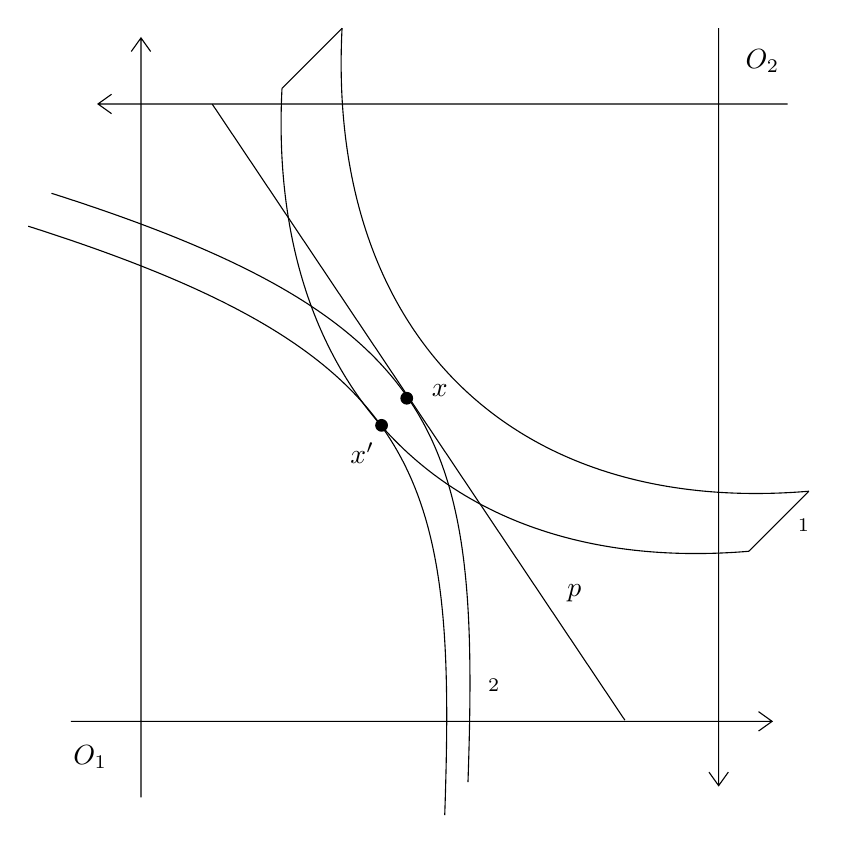
\begin{tikzpicture}[x=0.70pt,y=0.70pt,yscale=-1,xscale=1]
            %uncomment if require: \path (0,443); %set diagram left start at 0, and has height of 443

            %Shape: Axis 2D [id:dp22115699468612893] 
            \draw  (140,370.4) -- (502,370.4)(176.2,17.6) -- (176.2,409.6) (495,365.4) -- (502,370.4) -- (495,375.4) (171.2,24.6) -- (176.2,17.6) -- (181.2,24.6)  ;
            %Shape: Axis 2D [id:dp32207533916759135] 
            \draw  (510,51.7) -- (154,51.7)(474.4,403.6) -- (474.4,12.6) (161,56.7) -- (154,51.7) -- (161,46.7) (479.4,396.6) -- (474.4,403.6) -- (469.4,396.6)  ;
            %Curve Lines [id:da8559403196511832] 
            \draw    (249,43.6) .. controls (241,199.6) and (335,295.6) .. (490,282.6) ;
            %Curve Lines [id:da37662840950707166] 
            \draw    (280,12.6) .. controls (272,168.6) and (366,264.6) .. (521,251.6) ;
            %Straight Lines [id:da5642668535456735] 
            \draw    (249,43.6) -- (280,12.6) ;
            %Straight Lines [id:da9097139754709688] 
            \draw    (490,282.6) -- (521,251.6) ;
            %Curve Lines [id:da09819389723996741] 
            \draw    (130,97.8) .. controls (337,163.8) and (351,225.8) .. (345,401.8) ;
            %Shape: Circle [id:dp16582666368555876] 
            \draw  [fill={rgb, 255:red, 0; green, 0; blue, 0 }  ,fill opacity=1 ] (310.4,203.6) .. controls (310.4,201.94) and (311.74,200.6) .. (313.4,200.6) .. controls (315.06,200.6) and (316.4,201.94) .. (316.4,203.6) .. controls (316.4,205.26) and (315.06,206.6) .. (313.4,206.6) .. controls (311.74,206.6) and (310.4,205.26) .. (310.4,203.6) -- cycle ;
            %Shape: Circle [id:dp20605667579120546] 
            \draw  [fill={rgb, 255:red, 0; green, 0; blue, 0 }  ,fill opacity=1 ] (297.4,217.6) .. controls (297.4,215.94) and (298.74,214.6) .. (300.4,214.6) .. controls (302.06,214.6) and (303.4,215.94) .. (303.4,217.6) .. controls (303.4,219.26) and (302.06,220.6) .. (300.4,220.6) .. controls (298.74,220.6) and (297.4,219.26) .. (297.4,217.6) -- cycle ;
            %Curve Lines [id:da6954752398238686] 
            \draw    (118,114.8) .. controls (325,180.8) and (339,242.8) .. (333,418.8) ;
            %Straight Lines [id:da49767621503014337] 
            \draw    (213,51.8) -- (426,369.8) ;

            % Text Node
            \draw (140,381.4) node [anchor=north west][inner sep=0.75pt]    {$O_{1}$};
            % Text Node
            \draw (487,22.4) node [anchor=north west][inner sep=0.75pt]    {$O_{2}$};
            % Text Node
            \draw (514,264.4) node [anchor=north west][inner sep=0.75pt]    {$\succsim _{1}$};
            % Text Node
            \draw (325,195.4) node [anchor=north west][inner sep=0.75pt]    {$x$};
            % Text Node
            \draw (283,225.4) node [anchor=north west][inner sep=0.75pt]    {$x'$};
            % Text Node
            \draw (354,347.4) node [anchor=north west][inner sep=0.75pt]    {$\succsim _{2}$};
            % Text Node
            \draw (395,298.4) node [anchor=north west][inner sep=0.75pt]    {$p$};
        \end{tikzpicture}
        \caption{Local non-satiation is necessary for the First Welfare Theorem.}
        \label{fig:lns-welf}
    \end{center}
\end{figure}

\begin{techremark}
    Why can \(x\) be supported as a \usename{axn:weqt} in Figure~\ref{fig:lns-welf}?
\end{techremark}

Let us now interpret Theorem~\ref{thm:fftwe}. A classical economic question is how to allocate resources given information about preferences.\footnote{In its most general form, a question of this kind is asked in \cite{arrowSocialChoiceIndividual2012}, the spark that gave rise to modern social choice theory.} We might want such an allocation of resources to satisfy some attractive properties from a \textit{normative} perspective. One such property is Pareto optimality. An allocation rule that takes preferences and endowments as inputs and returns a \usename{axn:po} allocation as output might therefore be desirable. However, once one has an allocation rule, one might wonder whether it can be implemented in a decentralised way. A rule that maps preferences and endowments into an allocation does not, by itself, tell us \textit{how} to reach that allocation.

Theorem~\ref{thm:fftwe} tells us that Walrasian equilibrium with transfers implements an allocation rule that always delivers \usename{axn:po} allocations. Decentralised individual optimisation at some prices can therefore lead to desirable allocations from this point of view. There is a bit more, however. A Walrasian equilibrium with transfers is not just a mechanism to implement \usename{axn:po} allocations. It also induces a price for each good, which individuals can use to trade in order to reach those allocations. Prices may be interpreted as \textquote{values} for goods, where these values depend on the preferences and endowments of all individuals in the economy. In fact, \cite{debreuTheoryValueAxiomatic1959} is titled \textit{Theory of Value}.

Many more or less sophisticated critiques of economics stem from the idea that it is inappropriate to view the value of goods as determined by prices. There is a famous quotation, often misattributed to Oscar Wilde,\footnote{Apparently the original quotation is \textquote{[A cynic is] a man who knows the price of everything, and the value of nothing} from \citet[p. 55]{wildeLadyWindermeresFan1995}.} that says: \textquote{An economist is someone who knows the price of everything and the value of nothing}. Of course, there are legitimate reasons to question whether values should be entirely derived from individual preferences. But, in the setting we consider here, there is nothing special about prices that is not ultimately related to preferences or endowments.\footnote{However, sometimes the mere existence of prices, from a physical point of view, induces disgust towards the commodification of goods that \textquote{should not be priced}. As \citet[p. 201]{sophoclesAntigoneSophoclesEnglish1939} puts it: \textquote{There’s nothing in the world so demoralizing as money}. \cite{fleurbaeyEfficiencyEquitySociallyembedded2025} studies a class of problems, of which commodification is one, in a general equilibrium setting, so you are ready to read it!}

Unfortunately, an allocation rule that delivers \usename{axn:po} allocations can sometimes be undesirable from other points of view. For instance, it might deliver very unequal allocations. We might therefore want to complement Pareto optimality with a distributional requirement. One candidate is envy-freeness, which is closely related to the idea of equality of opportunity. One way to make this relationship precise is captured in the following proposition.

\begin{proposition}\label{prop:envy}
    Every allocation selected by \(R^{EW}\) satisfies \usename{axn:no-envy}. That is,

    \[
        x \in R^{EW}(E) \quad \Longrightarrow \quad x \ \text{satisfies \usename{axn:no-envy}}.
    \]
\end{proposition}

\begin{proof}
    Let \(E\) be an economy and suppose that \(x \in R^{EW}(E)\). By definition of \usename{axn:weqe}, there exists a price vector \(p \in \mathbb{R}^\ell_{++}\) such that, for each individual \(i\),

    \[
        x_i \in D_i\!\left(p,\frac{\bar e}{n}\right).
    \]

    Because all individuals face the same endowment \(\frac{\bar e}{n}\) and the same price vector \(p\), they all face the same budget set

    \[
        B := B\!\left(p, \frac{\bar e}{n}\right)
        = \left\{\, x_i' \in \mathbb{R}^\ell_+ \ \middle|\ p \cdot x_i' \le p \cdot \tfrac{\bar e}{n} \,\right\}.
    \]

    Fix any individual \(i\). Since \(x_i \in D_i\!\left(p,\frac{\bar e}{n}\right)\), \(x_i\) is a most preferred bundle for \(i\) in \(B\). Therefore,

    \begin{equation}
        \label{eq:maximal}
        \text{for all } x_i' \in B,\qquad x_i \succsim_i x_i'.
    \end{equation}

    Now consider any other individual \(j\neq i\). Since \(x_j \in D_j\!\left(p,\frac{\bar e}{n}\right)\), we have \(x_j \in B\). Applying \eqref{eq:maximal} to the specific bundle \(x_j\) yields

    \[
        x_i \succsim_i x_j.
    \]

    Since \(i\) and \(j\neq i\) were arbitrary, it follows that for all \(i\neq j\),

    \[
        x_i \succsim_i x_j,
    \]

    which is exactly \usename{axn:no-envy}. Hence the allocation \(x\) satisfies \usename{axn:no-envy}.
\end{proof}

Since any \usename{axn:weqe} is also a \usename{axn:weqt}, take transfers \(T_i := \tfrac{\bar e}{n} - e_i\), Theorem~\ref{thm:fftwe} and Proposition~\ref{prop:envy} together imply that the Egalitarian Walrasian allocation rule delivers allocations that are both \usename{axn:po} and satisfy \usename{axn:no-envy}. Therefore, in this simple setting, requirements of \textit{efficiency}, \textit{fairness}, and \textit{incentives} are not incompatible!\footnote{\citet[p. 405]{thomsonFairAllocationRules2011} discusses that the Egalitarian Walrasian allocation rule is also easy to implement under incomplete information about preferences.}

However, the actual endowments \(e_i\) need not coincide with the egalitarian endowment \(\tfrac{\bar e}{n}\). We might therefore be interested in understanding when such an allocation rule can be implemented starting from an arbitrary endowment profile. The second fundamental theorem of welfare economics, which we discuss in the next lecture, provides conditions under which this is possible.

\paragraph{Things to read.} The proof of Theorem~\ref{thm:fftwe} in these notes follows \citet[pp. 545--550]{mas-colellMicroeconomicTheory1995}. A proof of a closely related version of Proposition~\ref{prop:envy} appears in \citet[p. 46]{fleurbaeyFairnessResponsibilityWelfare2008}, which also discusses further properties of allocations satisfying \usename{axn:no-envy}.

\section{Exercises}

\begin{exercise}
    Explain why Proposition~\ref{prop:envy} links envy-freeness to equality of opportunity. There are at least a couple of things to say here. For instance, do the allocations selected by the Egalitarian Walrasian allocation rule depend on individuals' endowments?
\end{exercise}

\bibliographystyle{apacite}  % or another  style
\bibliography{references} % .bib file goes in ./bib/
\renewcommand{\thefootnote}{\fnsymbol{footnote}}

\chapter[Second theorem of welfare economics]%
 {Second theorem of welfare economics}%
\label{ch:L9}

% 3) Reset things so later footnotes go back to 1, 2, 3, …
%\setcounter{footnote}{0}
\renewcommand{\thefootnote}{\arabic{footnote}}

%\section{Separating hyperplane}\label{sec:L9-intro}

\begin{theorem}\label{thm:supporting-hyperplane} (\textbf{Separating hyperplane})
    Let \(B \subset \mathbb{R}^L\) be a convex set and let \(x \notin \operatorname{Int} B\)
    (the interior of \(B\)). Then there exists a nonzero vector \(p \in \mathbb{R}^L\) such that
    \[
        p \cdot x \;\ge\; p \cdot y \qquad \text{for every } y \in B.
    \]
    In words: there is a hyperplane through \(x\) that supports \(B\) from one side.
\end{theorem}

\begin{proof}
    We use the separating hyperplane theorem in the following form:

    \medskip
    \noindent
    \textit{Separating hyperplane theorem.}
    Let \(B \subset \mathbb{R}^L\) be convex and let \(z \notin \overline B\) (the
    closure of \(B\)). Then there exist \(p \in \mathbb{R}^L\) with \(p \neq 0\) and
    \(a \in \mathbb{R}\) such that
    \[
        p \cdot z \;>\; a \;\ge\; p \cdot y \qquad\text{for all } y \in B.
    \]
    \medskip

    Now take \(x \notin \operatorname{Int} B\). Then every neighbourhood of \(x\)
    contains points that are not in \(B\). In particular, we can find a sequence
    \((x^m)_{m\ge 1}\) such that
    \[
        x^m \to x \qquad\text{and}\qquad x^m \notin \overline B
        \quad\text{for all } m.
    \]
    (Think of \(x^m\) approaching \(x\) from “outside” \(B\).)

    For each \(m\), apply the separating hyperplane theorem to the convex set \(B\)
    and the point \(x^m \notin \overline B\). We obtain a nonzero vector
    \(p^m \in \mathbb{R}^L\) and a scalar \(c^m \in \mathbb{R}\) such that
    \begin{equation}\label{eq:sep-m}
        p^m \cdot x^m \;>\; c^m \;\ge\; p^m \cdot y
        \qquad\text{for all } y \in B.
    \end{equation}

    Normalize the vectors \(p^m\) so that \(\|p^m\| = 1\) for every \(m\) (we can always
    divide \(p^m\) and \(c^m\) by the same positive constant without changing the
    inequalities). The sequence \((p^m)\) lives on the unit sphere, which is compact,
    so there is a subsequence (still denoted \((p^m)\) for simplicity) that converges:
    \[
        p^m \to p \qquad\text{for some } p \in \mathbb{R}^L \text{ with } \|p\|=1.
    \]
    In particular \(p \neq 0\). Since \((c^m)\) is a sequence of real numbers, we can
    also extract a further subsequence (again not relabelled) such that
    \[
        c^m \to c \qquad\text{for some } c \in \mathbb{R}.
    \]

    Fix any \(y \in B\). Inequality \eqref{eq:sep-m} gives, for each \(m\),
    \[
        p^m \cdot x^m \;>\; c^m \;\ge\; p^m \cdot y.
    \]
    Taking limits as \(m\to\infty\) and using continuity of the dot product,
    and the convergences \(x^m \to x\), \(p^m \to p\) and \(c^m \to c\), we obtain
    \[
        p \cdot x \;\ge\; c \;\ge\; p \cdot y.
    \]
    Since this holds for every \(y \in B\), we have
    \[
        p \cdot x \;\ge\; p \cdot y \qquad\text{for all } y \in B,
    \]
    which is exactly the desired supporting hyperplane inequality.
\end{proof}

%\section{The welfare theorem}

\begin{theorem}\label{thm:sftwe} (\textbf{Second fundamental theorem of welfare economics}) If preferences in the economy \( E \) are locally non-satiated, convex, and continuous, and endowments are strictly positive \( e_i \in \mathbb{R}^\ell_{++} \) for all individuals \( i \), then every interior Pareto optimal allocation \( x \in \mathbb{R}^{\ell n}_{++}\) can be supported as a Walrasian equilibrium with transfers. That is,

    \[
        x \quad \text{is Pareto optimal} \quad \Longrightarrow \quad x \in R^{WT}(E).
    \]
\end{theorem}

\begin{proof}
    Say we want to implement the interior Pareto optimal allocation \( x \). Define transfers \( T_i \) by

    \[
        T_i = x_i - e_i \qquad\text{for each } i.
    \]

    Feasibility of \( x \) implies \( \sum_{i} x_i = \sum_{i} e_i \), hence \( \sum_{i} T_i = 0 \), so \( (T_i)_{i} \) is a feasible vector of lump–sum transfers. We have to find strictly positive prices \( p \) such that for each individual, endowed with \( e_i+T_i = x_i \), the bundle \( x_i \) is in the Walrasian demand of \( i \):

    \[
        x_i \in D_i(p, e_i+T_i ) \qquad\text{for each } i.
    \]

    \paragraph{Step 1: “Strictly better–than” sets.}

    For each individual \( i \), let

    \[
        \overline{U}^i(x_i) := \{x'_i : x'_i \succ_i x_i\}
    \]

    denote the \textbf{strict} upper contour set at \( x_i \). By continuity and convexity of \( \succsim_i \) this set is convex, and \( x_i \notin \overline{U}^i(x_i) \). Define the set of aggregate improvements

    \[
        \overline{U} (x) = \sum_i \overline{U}^i (x)
        :=
        \Bigl\{\sum_{i} x'_i \in \mathbb{R}^{\ell}_{++} \;\Big|\; x'_i \in \overline{U}^i(x_i)\text{ for each }i\Bigr\}.
    \]

    So \( \overline{U}(x) \) is the set of all aggregate bundles that can be obtained by letting each individual choose a bundle strictly preferred to her allocation in \( x \). Since it is the sum of convex sets, \( \overline{U} (x) \) is convex. Pareto optimality of \( x \) says that there is no feasible allocation \( x'=(x'_i)_{i} \) with \( x'_i \succ_i x_i \) for all \( i \). Equivalently,

    \[
        \sum_{i} x_i \notin \overline{U} (x).
    \]

    \paragraph{Step 2: A supporting price hyperplane.}
    We have a convex set \( \overline{U}(x) \) and a point \( \sum_i x_i \) outside it. By the supporting hyperplane theorem, there exists a nonzero vector \( p \in \mathbb{R}^\ell_{+} \) such that

    \[
        p \cdot x' \;\ge\; p \cdot \Bigl(\sum_{i} x_i\Bigr)
        \qquad\text{for all } x' \in \overline{U}(x).
    \]

    In particular, for any profile \( (x'_i)_{i} \) with \( x'_i \in \overline{U}^i(x_i) \) for all \( i \),

    \begin{equation}\label{eq:sftwe}
        \sum_{i} p\cdot x'_i
        =
        p \cdot \Bigl(\sum_{i} x'_i\Bigr)
        \;\ge\;
        p \cdot \Bigl(\sum_{i} x_i\Bigr)
        =
        \sum_{i} p\cdot x_i.
    \end{equation}

    \paragraph{Step 3: Prices must be strictly positive.}
    We now show that prices are strictly positive, i.e., \( p \in \mathbb{R}^\ell_{++} \).

    \emph{(i) No component of \( p \) can be negative.} Suppose \( p_\ell < 0 \) for some \( \ell \). Pick any individual \( i \). By monotonicity, for any small \( \varepsilon>0 \) the bundle

    \[
        x'_i := x_i + \varepsilon e_\ell
    \]

    satisfies \( x'_i \succ_i x_i \), hence \( x'_i \in \overline{U}^i(x_i) \), while all
    other individuals \( j\neq i \) keep \( x'_j = x_j \). Thus \( x' := \sum_i x'_i \in \overline{U}(x) \). By the supporting hyperplane inequality from Step~2,

    \[
        p\cdot x' \;\ge\; p\cdot \sum_i x_i.
    \]

    But

    \[
        p\cdot x'
        =
        p\cdot \sum_i x_i + \varepsilon p_\ell
        <
        p\cdot \sum_i x_i,
    \]

    a contradiction. Hence \( p_\ell \ge 0 \) for each \( \ell \), so \( p \in \mathbb{R}^\ell_{+} \).

    \emph{(ii) No component of \( p \) can be zero.} Suppose \( p_\ell = 0 \) for some \( \ell \). Again choose any individual \( i \). Because \(x_i \in \mathbb{R}^\ell_{++}\), there is some small \( \varepsilon>0 \) such that \(x_i - \varepsilon \mathbf{1} \in \mathbb{R}^\ell_{+}\), where \(\mathbf{1}\) is the vector of all ones. Consider bundles \(y_i\) of the form

    \[
        y^i_\ell > x^i_\ell,
        \qquad
        y^i_{k} = x^i_{k} - \varepsilon
        \ \text{ for all } k \neq \ell.
    \]

    By continuity and monotonicity of preferences, we can choose \(y_i\) of this form (with \(\varepsilon\) small and \(y^i_\ell\) large enough) so that \( y_i \succ_i x_i \), hence \(y_i \in \overline{U}^i(x_i)\). For all \( j\neq i \), set \( y_j := x_j \). Then \( y := \sum_j y_j \in \overline{U}(x) \), so Step~2 gives

    \[
        p\cdot y \;\ge\; p\cdot \sum_j x_j.
    \]

    But

    \[
        p\cdot y
        =
        p\cdot \sum_j x_j
        +
        \sum_{k\neq \ell} (y^i_k - x^i_k) p_k
        +
        (y^i_\ell - x^i_\ell)p_\ell.
    \]

    Here \(y^i_k - x^i_k = -\varepsilon <0\) for all \(k\neq \ell\) and \(p_k \ge 0\), while \(p_\ell = 0\). Since \(p\neq 0\), at least one of the \(p_k\) with \(k\neq \ell\) is strictly positive, so

    \[
        \sum_{k\neq \ell} (y^i_k - x^i_k) p_k < 0,
    \]

    and hence \(p\cdot y < p\cdot \sum_j x_j\), a contradiction. Therefore no component of \(p\) can be zero either, and we conclude that \(p \in \mathbb{R}^\ell_{++}\).

    \paragraph{Step 4: Individual optimality.} Fix an individual \(i\). We show that \(x_i\) is optimal in her budget set. Suppose, by contradiction, that there exists \(x'_i \in \overline{U}^i(x_i)\) with \(p\cdot x'_i \le p\cdot x_i\). Keep all other individuals at their original bundles: \(x'_j := x_j\) for every \(j\neq i\). Then the profile \((x'_k)_k\) satisfies \(x'_k \in \overline{U}^k(x_k)\) for all \(k\), so \(\sum_k x'_k \in \overline{U}(x)\). By Equation \eqref{eq:sftwe} we must have

    \[
        \sum_k p\cdot x'_k \;\ge\; \sum_k p\cdot x_k.
    \]

    On the other hand,

    \[
        \sum_k p\cdot x'_k
        =
        p\cdot x'_i + \sum_{j\neq i} p\cdot x_j
        \le
        p\cdot x_i + \sum_{j\neq i} p\cdot x_j
        =
        \sum_k p\cdot x_k,
    \]

    with strict inequality if \(p\cdot x'_i < p\cdot x_i\). This contradicts \eqref{eq:sftwe}. Hence no such \(x'_i\) exists, and \(x_i\) is optimal at prices \(p\), that is,

    \[
        x_i \in D_i(p, e_i+T_i).
    \]

    \paragraph{Conclusion.}
    We have found prices \(p \in \mathbb{R}^\ell_{++}\) and transfers \((T_i)_i\) such that
    \[
        x_i \in D_i(p, e_i+T_i)\qquad\text{for all } i.
    \]
    Hence \(x\) is a Walrasian equilibrium with transfers: \(x \in R^{WT}(E)\). Since \(x\) was an arbitrary interior Pareto optimal allocation, the theorem follows.
\end{proof}

\paragraph{Things to read.} This lecture is based on \citet[pp. 545-550]{mas-colellMicroeconomicTheory1995}.

\section{Exercises}

hey.

\bibliographystyle{apacite}  % or another  style
\bibliography{references} % .bib file goes in ./bib/
\renewcommand{\thefootnote}{\fnsymbol{footnote}}

\chapter[Existence of competitive equilibria]%
 {Existence of competitive equilibria}%
\label{ch:L10}

% 3) Reset things so later footnotes go back to 1, 2, 3, …
%\setcounter{footnote}{0}
\renewcommand{\thefootnote}{\arabic{footnote}}

We assume preferences are continuous, strictly convex, and strongly monotone. Under these assumptions, we can prove that a competitive equilibrium exists.

\begin{definition}
    A preference relation is \textbf{strongly monotone} if for all \(x, y \in \mathbb{R}^L_+\) such that \(x \geq y\) and \(x \neq y\), we have \(x \succ y\).
\end{definition}

\begin{definition}
    A preference relation is \textbf{strictly convex} if for all \(x, y, z \in \mathbb{R}^L_+\) such that \(y \succ x\) and \(z \succ x\), we have for all \(\alpha \in (0,1)\), \(\alpha y + (1-\alpha) z \succ x\). Equivalently, all upper contour sets are strictly convex sets.
\end{definition}

If a preference relation is continuous, strictly convex, and strongly monotone, then the Walrasian demand is single-valued and can therefore be viewed as a function. We can then define the excess demand function as follows.

\begin{definition}
    The \textbf{excess demand function} of and individual \( i \) with a single-valued Walrasian demand function \( D_i(p, e_i) \) is given by
    \[z_i(p, e_i) = D_i(p, e_i) - e_i.\]
\end{definition}

From the individual excess demand functions, we can construct the aggregate excess demand function.

\[
    z(p) = \sum_i z_i (p) .
\]

The excess demand function maps prices to allocations. Under our assumptions on preferences, Walrasian equilibrium can be characterised through the excess demand function as follows.

\begin{proposition}\label{prop:walr_excess}
    If individual preferences \( \succsim_i \) are continuous, strictly convex, and strongly monotone for each \( i \), then an allocation \( x \) is a Walrasian equilibrium if and only if there exists a price vector \( p \) such that \( z (p) = 0 \).
\end{proposition}

The excess demand function has several important properties that we will use to prove the existence of a competitive equilibrium.

\begin{proposition}\label{prop:excess}
    If individual preferences \( \succsim_i \) are continuous, strictly convex, and strongly monotone for each \( i \), then the aggregate excess demand function \( z(p) \) satisfies the following properties:
    \begin{enumerate}
        \item \( z(p) \) is \textbf{homogeneous of degree zero}:\( z( \alpha p) = z(p) \) for all \( \alpha > 0 \);
        \item \( z(p) \) satisfies Walras' law: \( p \cdot z(p) = 0 \) for all strictly positive prices \( p \);
        \item \( z(p) \) is continuous;
        \item there is an \( s > 0 \) such that for all goods \( \ell \) and prices \( p \), \( z_{\ell} (p) > -s \);
        \item if \(p^n \) is a sequence of prices converging to \( p \) with \( p_{\ell} = 0 \) for some good \( \ell \), then \( \max \{ z^1 (p^n), \ldots, z^L (p^n) \} \to +\infty \).
    \end{enumerate}
\end{proposition}

\begin{theorem}\label{thm:kaku} (\textbf{Kakutani's fixed point})
    Let \( A \subseteq \mathbb{R}^L \) be a non-empty, compact, and convex set, and \( f : A \rightrightarrows A \) be an upper hemicontinuous correspondence such that \( f(x) \subseteq A \) is non-empty and convex for each \( x \in A \). Then, \( f \) has a fixed point, i.e., there exists \( x \in A \) such that \( x \in f(x) \).
\end{theorem}

\begin{proposition}
    If the aggregate excess demand function \( z(p) \) satisfies the properties in Proposition \ref{prop:excess}, then there exists a price vector \( p \) such that \( z(p) = 0 \). Therefore, in such economy a Walrasian equilibrium exists.
\end{proposition}

\begin{proof}
    Because \( z(\cdot) \) is homogeneous of degree zero we can restrict attention to prices on the \emph{unit simplex}

    \[
        \Delta
        :=
        \Bigl\{
        p \in \mathbb{R}^\ell_+ \;\Bigm|\;
        \sum_{\ell=1}^\ell p^\ell = 1
        \Bigr\}.
    \]

    Let

    \[
        \text{Interior }\Delta
        :=
        \{ p \in \Delta : p^\ell > 0 \text{ for all } \ell \}
        \quad\text{and}\quad
        \text{Boundary }\Delta := \Delta \setminus \text{Interior }\Delta .
    \]

    Recall that \( z(\cdot) \) was originally defined for strictly positive
    prices only; by continuity, we can extend it uniquely to \( \Delta \).

    We construct a correspondence
    \( f : \Delta \rightrightarrows \Delta \) and then apply Kakutani's
    fixed–point theorem to \( f \). For notational simplicity, whenever
    \( q \in f(p) \) we write just ``\( q \)'' for such a vector.

    \paragraph{Step 1. Construction on Interior \( \Delta \).}
    For \( p \in \text{Interior }\Delta \) and \( p>0 \), define
    \[
        f(p)
        :=
        \bigl\{
        q \in \Delta
        \;\bigm|\;
        z(p)\cdot q \ge z(p)\cdot q'
        \text{ for all } q' \in \Delta
        \bigr\}.
    \]
    In words, given the current ``proposal'' \( p \), the correspondence
    \( f(\cdot) \) selects price vectors \( q \) that, among all admissible price
    vectors on the simplex, maximise the value of the (aggregate) excess
    demand vector \( z(p) \).

    Write \( z^\ell(p) \) for the excess demand of good \( \ell \) at prices \( p \).
    From the definition of \( f(p) \) one easily checks that
    \[
        f(p)
        =
        \Bigl\{
        q \in \Delta
        \;\Bigm|\;
        q^\ell = 0
        \text{ whenever }
        z^\ell(p) < \max\{ z^1(p),\dots,z^\ell(p)\}
        \Bigr\}.
    \]
    Indeed, if \( q \) put positive weight on some good with strictly lower
    excess demand than the maximum, we could reallocate that weight
    towards a good with maximal excess demand and increase
    \( z(p)\cdot q \), contradicting optimality of \( q \).

    By Walras' law, \( p \cdot z(p) = 0 \) for all strictly positive \( p \).
    Hence if \( z(p)\neq 0 \), at least one component of \( z(p) \) is negative
    and at least one is positive, so the maximum of the components is
    strictly positive. In that case, every \( q\in f(p) \) has \( q^\ell=0 \) for
    some \( \ell \), so \( f(p) \subseteq \text{Boundary }\Delta \).
    In contrast, if \( z(p)=0 \), then \( z(p)\cdot q = 0 \) for all \( q \in \Delta \),
    so every \( q\in\Delta \) is a maximiser and \( f(p)=\Delta \).

    \paragraph{Step 2. Construction on Boundary \( \Delta \).}
    For \( p \in \text{Boundary }\Delta \), define
    \[
        f(p)
        :=
        \{ q \in \Delta : p\cdot q = 0 \}
        =
        \{ q \in \Delta : q^\ell = 0 \text{ whenever } p^\ell > 0 \}.
    \]
    Because \( p \) has at least one component equal to zero, this set is not
    empty: we can place all the weight of \( q \) on goods whose price is
    zero under \( p \).

    Note that with this construction no price vector on
    \( \text{Boundary }\Delta \) can be a fixed point of \( f(\cdot) \).
    Indeed, if \( p \in \text{Boundary }\Delta \) and \( p \in f(p) \), then
    we would have \( p\cdot p = 0 \), which is impossible because
    \( p \in \Delta \) implies \( p\cdot p>0 \).

    \paragraph{Step 3. Any fixed point of \( f \) is an equilibrium price.}
    Suppose that \( p^* \in \Delta \) is a fixed point of \( f \), i.e.
    \( p^* \in f(p^*) \).
    From Step~2 we know that no point on \( \text{Boundary }\Delta \) can be a
    fixed point, so we must have \( p^* \notin \text{Boundary }\Delta \),
    that is, \( p^* \in \text{Interior }\Delta \) and \( p^* > 0 \).

    If \( z(p^*) \neq 0 \), then Step~1 tells us that
    \( f(p^*) \subseteq \text{Boundary }\Delta \), so \( p^* \) cannot belong to
    \( f(p^*) \), a contradiction.
    Hence it must be that \( z(p^*) = 0 \).
    In other words, any fixed point of \( f(\cdot) \) is a price vector with
    zero aggregate excess demand.

    \paragraph{Step 4. The correspondence \( f \) is convex–valued and upper hemicontinuous.}
    \emph{Convex–valuedness.}
    When \( p \in \text{Interior }\Delta \), the set \( f(p) \) is the set of
    maximisers of a linear function \( q \mapsto z(p)\cdot q \) over the
    convex set \( \Delta \), hence it is convex.
    When \( p \in \text{Boundary }\Delta \), the set
    \( f(p) = \{q \in \Delta : p\cdot q=0\} \) is the intersection of the
    simplex \( \Delta \) with a linear subspace, and is therefore convex.
    Thus \( f(p) \) is convex for all \( p\in\Delta \).

    \smallskip
    \emph{Upper hemicontinuity.}
    Take any sequence \( p^n \to p \) in \( \Delta \) and a sequence
    \( q^n \in f(p^n) \) with \( q^n \to q \).
    We must show that \( q \in f(p) \).

    \medskip
    \noindent
    \textit{Case 1: \( p \in \text{Interior }\Delta \).}
    For \( n \) large enough, \( p^n \) is also in \( \text{Interior }\Delta \) and
    \( q^n \) maximises \( z(p^n)\cdot q \) over \( q\in\Delta \).
    The continuity of \( z(\cdot) \) gives \( z(p^n)\to z(p) \), and a standard
    argument for maximisers of continuous linear functionals on compact
    sets shows that any limit point of maximisers is a maximiser.
    Hence \( q \) maximises \( z(p)\cdot q \) over \( \Delta \), i.e.\ \( q \in f(p) \).

    \medskip
    \noindent
    \textit{Case 2: \( p \in \text{Boundary }\Delta \).}
    We need to show that \( p\cdot q = 0 \).
    Pick any good \( \ell \) with \( p^\ell>0 \).
    For \( n \) large enough we have \( p^{n,\ell} > 0 \) as well.

    First suppose that \( p^n \in \text{Boundary }\Delta \) for all large \( n \).
    Then by the definition of \( f(p^n) \) we have \( p^n\cdot q^n = 0 \) for
    such \( n \). Taking limits yields \( p\cdot q = 0 \).

    The more delicate case is when some \( p^n \) lie in
    \( \text{Interior }\Delta \) and converge to \( p \) on Boundary \( \Delta \).
    For those \( n \), \( q^n \) maximises \( z(p^n)\cdot q \) over \( \Delta \).
    We claim that, for large \( n \), \( q^{n,\ell}=0 \) whenever \( p^\ell>0 \).
    Once this is shown, passing to the limit gives \( q^\ell = 0 \) for all
    \( \ell \) with \( p^\ell>0 \), and hence \( p\cdot q = 0 \).

    Fix such an \( \ell \) with \( p^\ell>0 \).
    Because \( p^\ell>0 \), there is an \( \varepsilon>0 \) such that
    \( p^{n,\ell} \ge \varepsilon \) for all large \( n \).
    For those \( n \), optimality of \( q^n \) implies
    \[
        z^\ell(p^n)
        \le \max_k z^k(p^n),
    \]
    and by property~(v) of Proposition~\ref{prop:excess},
    the right–hand side tends to \( +\infty \) as \( n\to\infty \)
    whenever \( p^n \) approaches the boundary.
    On the other hand, the lower bound on excess demand in
    property~(iv) bounds \( z^\ell(p^n) \) from below, and
    Walras' law implies
    \[
        z^\ell(p^n)
        = - \frac{1}{p^{n,\ell}}
        \sum_{r\neq \ell} p^{n,r} z^r(p^n)
        \le \frac{s}{\varepsilon},
    \]
    where \( s>0 \) is the bound from property~(iv).
    Thus \( z^\ell(p^n) \) is bounded above, which is only compatible with
    property~(v) if \( q^{n,\ell}=0 \) for all large \( n \).
    (Intuitively, as \( p^n \) approaches the boundary, any maximal excess
    demand must be concentrated on goods whose prices go to zero.)

    We conclude that in the limit \( q \) assigns positive weight only to
    goods whose prices under \( p \) are zero, so \( p\cdot q = 0 \) and hence
    \( q \in f(p) \).

    In both cases \( q \in f(p) \), so \( f \) is upper hemicontinuous.

    \paragraph{Step 5. Existence of a fixed point.}
    The simplex \( \Delta \) is nonempty, compact, and convex.
    By the previous step, the correspondence
    \( f : \Delta \rightrightarrows \Delta \) has nonempty, convex values
    and is upper hemicontinuous.
    Theorem \ref{thm:kaku} therefore guarantees the existence of
    a fixed point \( p^* \in \Delta \) with \( p^* \in f(p^*) \).

    By Step~3, any such fixed point satisfies \( z(p^*) = 0 \).
    Hence there exists a price vector \( p^* \in \mathbb{R}^\ell_{++} \) such
    that \( z(p^*) = 0 \).
    By Proposition~\ref{prop:walr_excess}, this means that a Walrasian
    equilibrium exists.
\end{proof}

\paragraph{Things to read.} This lecture is based on \citet[pp. 578-586]{mas-colellMicroeconomicTheory1995}.

\section{Exercises}

\begin{exercise}
    Show that if demand equals supply in \( k-1 \) markets, then it also equals supply in the \( k \)-th market. (Hint: Use Walras' law.)
\end{exercise}

\begin{exercise}
    Prove Proposition \ref{prop:walr_excess}.
\end{exercise}

\begin{exercise}
    Prove property 1. of the excess demand function in Proposition \ref{prop:excess}.
\end{exercise}

\bibliographystyle{apacite}  % or another  style
\bibliography{references} % .bib file goes in ./bib/

%\appendix

% — Appendix to Chapter 1 —
%\include{appendices/1_universalisation_appendix}


% --------------------------------------------------------------------
\end{document}